\documentclass[11pt,fleqn]{book} % Default font size and left-justified equations
%%%%%%%%%%%%%%%%%%%%%%%%%%%%%%%%%%%%%%%%%
% The Legrand Orange Book
% LaTeX Template
% Version 2.0 (9/2/15)
%%%%%%%%%%%%%%%%%%%%%%%%%%%%%%%%%%%%%%%%%%
%  Adaptado por Prof. Ausberto Castro Vera,
%  2013-2021
%----------------------------------------------------------------------------------------
%	PACKAGES AND OTHER DOCUMENT CONFIGURATIONS
%----------------------------------------------------------------------------------------

%%%%%%%%%%%%%%%%%%%%%%%%%%%%%%%%%%%%%%%%%
% The Legrand Orange Book
% Structural Definitions File
% Version 2.0 (9/2/15)
%
% Original author:
% Mathias Legrand (legrand.mathias@gmail.com) with modifications by:
% Vel (vel@latextemplates.com)
%
% This file has been downloaded from:
% http://www.LaTeXTemplates.com
%
% License:
% CC BY-NC-SA 3.0 (http://creativecommons.org/licenses/by-nc-sa/3.0/)
%
%%%%%%%%%%%%%%%%%%%%%%%%%%%%%%%%%%%%%%%%%%

%----------------------------------------------------------------------------------------
%	VARIOUS REQUIRED PACKAGES AND CONFIGURATIONS
%----------------------------------------------------------------------------------------

\usepackage[top=3cm,bottom=3cm,left=3cm,right=3cm,headsep=10pt,a4paper]{geometry} % Page margins

\usepackage{graphicx} % Required for including pictures
\graphicspath{{Pictures/}} % Specifies the directory where pictures are stored

\usepackage{lipsum} % Inserts dummy text
\usepackage{here}   %
\usepackage{tikz} % Required for drawing custom shapes

\usepackage[brazil]{babel} % Brazilian Portuguese language/hyphenation

\usepackage{enumitem} % Customize lists
\setlist{nolistsep} % Reduce spacing between bullet points and numbered lists

\usepackage{booktabs} % Required for nicer horizontal rules in tables

\usepackage{xcolor} % Required for specifying colors by name
\definecolor{ocre}{RGB}{243,102,25} % Define the orange color used for highlighting throughout the book

%----------------------------------------------------------------------------------------
%	FONTS
%----------------------------------------------------------------------------------------

\usepackage{avant} % Use the Avantgarde font for headings
%\usepackage{times} % Use the Times font for headings
\usepackage{mathptmx} % Use the Adobe Times Roman as the default text font together with math symbols from the Sym­bol, Chancery and Com­puter Modern fonts

\usepackage{microtype} % Slightly tweak font spacing for aesthetics
\usepackage[utf8]{inputenc} % Required for including letters with accents
\usepackage[T1]{fontenc} % Use 8-bit encoding that has 256 glyphs

%----------------------------------------------------------------------------------------
%	BIBLIOGRAPHY AND INDEX
%----------------------------------------------------------------------------------------
\usepackage{hyperref}

%\usepackage[style=alphabetic, citestyle=numeric, sorting=nyt, sortcites=true,
%            autopunct=true, babel=hyphen, hyperref=true, abbreviate=false,
%            backref=true, backend=biber]{biblatex}
%\addbibresource{racketbib.bib} % BibTeX bibliography file
%\defbibheading{bibempty}{}

\usepackage{calc} % For simpler calculation - used for spacing the index letter headings correctly
\usepackage{makeidx} % Required to make an index
\makeindex % Tells LaTeX to create the files required for indexing

%----------------------------------------------------------------------------------------
%	MAIN TABLE OF CONTENTS
%----------------------------------------------------------------------------------------

\usepackage{titletoc} % Required for manipulating the table of contents

\contentsmargin{0cm} % Removes the default margin

% Part text styling
\titlecontents{part}[0cm]
{\addvspace{20pt}\centering\large\bfseries}
{}
{}
{}

% Chapter text styling
\titlecontents{chapter}[1.25cm] % Indentation
{\addvspace{12pt}\large\sffamily\bfseries} % Spacing and font options for chapters
{\color{ocre!60}\contentslabel[\Large\thecontentslabel]{1.25cm}\color{ocre}} % Chapter number
{\color{ocre}}
{\color{ocre!60}\normalsize\;\titlerule*[.5pc]{.}\;\thecontentspage} % Page number

% Section text styling
\titlecontents{section}[1.25cm] % Indentation
{\addvspace{3pt}\sffamily\bfseries} % Spacing and font options for sections
{\contentslabel[\thecontentslabel]{1.25cm}} % Section number
{}
{\hfill\color{black}\thecontentspage} % Page number
[]

% Subsection text styling
\titlecontents{subsection}[1.25cm] % Indentation
{\addvspace{1pt}\sffamily\small} % Spacing and font options for subsections
{\contentslabel[\thecontentslabel]{1.25cm}} % Subsection number
{}
{\ \titlerule*[.5pc]{.}\;\thecontentspage} % Page number
[]

% List of figures
\titlecontents{figure}[0em]
{\addvspace{-5pt}\sffamily}
{\thecontentslabel\hspace*{1em}}
{}
{\ \titlerule*[.5pc]{.}\;\thecontentspage}
[]

% List of tables
\titlecontents{table}[0em]
{\addvspace{-5pt}\sffamily}
{\thecontentslabel\hspace*{1em}}
{}
{\ \titlerule*[.5pc]{.}\;\thecontentspage}
[]

%----------------------------------------------------------------------------------------
%	MINI TABLE OF CONTENTS IN PART HEADS
%----------------------------------------------------------------------------------------

% Chapter text styling
\titlecontents{lchapter}[0em] % Indenting
{\addvspace{15pt}\large\sffamily\bfseries} % Spacing and font options for chapters
{\color{ocre}\contentslabel[\Large\thecontentslabel]{1.25cm}\color{ocre}} % Chapter number
{}
{\color{ocre}\normalsize\sffamily\bfseries\;\titlerule*[.5pc]{.}\;\thecontentspage} % Page number

% Section text styling
\titlecontents{lsection}[0em] % Indenting
{\sffamily\small} % Spacing and font options for sections
{\contentslabel[\thecontentslabel]{1.25cm}} % Section number
{}
{}

% Subsection text styling
\titlecontents{lsubsection}[.5em] % Indentation
{\normalfont\footnotesize\sffamily} % Font settings
{}
{}
{}

%----------------------------------------------------------------------------------------
%	PAGE HEADERS
%----------------------------------------------------------------------------------------

\usepackage{fancyhdr} % Required for header and footer configuration

\pagestyle{fancy}
\renewcommand{\chaptermark}[1]{\markboth{\sffamily\normalsize\bfseries\chaptername\ \thechapter.\ #1}{}} % Chapter text font settings
\renewcommand{\sectionmark}[1]{\markright{\sffamily\normalsize\thesection\hspace{5pt}#1}{}} % Section text font settings
\fancyhf{} \fancyhead[LE,RO]{\sffamily\normalsize\thepage} % Font setting for the page number in the header
\fancyhead[LO]{\rightmark} % Print the nearest section name on the left side of odd pages
\fancyhead[RE]{\leftmark} % Print the current chapter name on the right side of even pages
\renewcommand{\headrulewidth}{0.5pt} % Width of the rule under the header
\addtolength{\headheight}{2.5pt} % Increase the spacing around the header slightly
\renewcommand{\footrulewidth}{0pt} % Removes the rule in the footer
\fancypagestyle{plain}{\fancyhead{}\renewcommand{\headrulewidth}{0pt}} % Style for when a plain pagestyle is specified

% Removes the header from odd empty pages at the end of chapters
\makeatletter
\renewcommand{\cleardoublepage}{
\clearpage\ifodd\c@page\else
\hbox{}
\vspace*{\fill}
\thispagestyle{empty}
\newpage
\fi}

%----------------------------------------------------------------------------------------
%	THEOREM STYLES
%----------------------------------------------------------------------------------------

\usepackage{amsmath,amsfonts,amssymb,amsthm} % For math equations, theorems, symbols, etc

\newcommand{\intoo}[2]{\mathopen{]}#1\,;#2\mathclose{[}}
\newcommand{\ud}{\mathop{\mathrm{{}d}}\mathopen{}}
\newcommand{\intff}[2]{\mathopen{[}#1\,;#2\mathclose{]}}
\newtheorem{notation}{Notation}[chapter]

% Boxed/framed environments
\newtheoremstyle{ocrenumbox}% % Theorem style name
{0pt}% Space above
{0pt}% Space below
{\normalfont}% % Body font
{}% Indent amount
{\small\bf\sffamily\color{ocre}}% % Theorem head font
{\;}% Punctuation after theorem head
{0.25em}% Space after theorem head
{\small\sffamily\color{ocre}\thmname{#1}\nobreakspace\thmnumber{\@ifnotempty{#1}{}\@upn{#2}}% Theorem text (e.g. Theorem 2.1)
\thmnote{\nobreakspace\the\thm@notefont\sffamily\bfseries\color{black}---\nobreakspace#3.}} % Optional theorem note
\renewcommand{\qedsymbol}{$\blacksquare$}% Optional qed square

\newtheoremstyle{blacknumex}% Theorem style name
{5pt}% Space above
{5pt}% Space below
{\normalfont}% Body font
{} % Indent amount
{\small\bf\sffamily}% Theorem head font
{\;}% Punctuation after theorem head
{0.25em}% Space after theorem head
{\small\sffamily{\tiny\ensuremath{\blacksquare}}\nobreakspace\thmname{#1}\nobreakspace\thmnumber{\@ifnotempty{#1}{}\@upn{#2}}% Theorem text (e.g. Theorem 2.1)
\thmnote{\nobreakspace\the\thm@notefont\sffamily\bfseries---\nobreakspace#3.}}% Optional theorem note

\newtheoremstyle{blacknumbox} % Theorem style name
{0pt}% Space above
{0pt}% Space below
{\normalfont}% Body font
{}% Indent amount
{\small\bf\sffamily}% Theorem head font
{\;}% Punctuation after theorem head
{0.25em}% Space after theorem head
{\small\sffamily\thmname{#1}\nobreakspace\thmnumber{\@ifnotempty{#1}{}\@upn{#2}}% Theorem text (e.g. Theorem 2.1)
\thmnote{\nobreakspace\the\thm@notefont\sffamily\bfseries---\nobreakspace#3.}}% Optional theorem note

% Non-boxed/non-framed environments
\newtheoremstyle{ocrenum}% % Theorem style name
{5pt}% Space above
{5pt}% Space below
{\normalfont}% % Body font
{}% Indent amount
{\small\bf\sffamily\color{ocre}}% % Theorem head font
{\;}% Punctuation after theorem head
{0.25em}% Space after theorem head
{\small\sffamily\color{ocre}\thmname{#1}\nobreakspace\thmnumber{\@ifnotempty{#1}{}\@upn{#2}}% Theorem text (e.g. Theorem 2.1)
\thmnote{\nobreakspace\the\thm@notefont\sffamily\bfseries\color{black}---\nobreakspace#3.}} % Optional theorem note
\renewcommand{\qedsymbol}{$\blacksquare$}% Optional qed square
\makeatother

% Defines the theorem text style for each type of theorem to one of the three styles above
\newcounter{dummy}
\numberwithin{dummy}{section}
\theoremstyle{ocrenumbox}
\newtheorem{theoremeT}[dummy]{Theorem}
\newtheorem{problem}{Problem}[chapter]
\newtheorem{exerciseT}{Exercise}[chapter]
\theoremstyle{blacknumex}
\newtheorem{exampleT}{Example}[chapter]
\theoremstyle{blacknumbox}
\newtheorem{vocabulary}{Vocabulary}[chapter]
\newtheorem{definitionT}{Definition}[section]
\newtheorem{corollaryT}[dummy]{Corollary}
\theoremstyle{ocrenum}
\newtheorem{proposition}[dummy]{Proposition}

%----------------------------------------------------------------------------------------
%	DEFINITION OF COLORED BOXES
%----------------------------------------------------------------------------------------

\RequirePackage[framemethod=default]{mdframed} % Required for creating the theorem, definition, exercise and corollary boxes

% Theorem box
\newmdenv[skipabove=7pt,
skipbelow=7pt,
backgroundcolor=black!5,
linecolor=ocre,
innerleftmargin=5pt,
innerrightmargin=5pt,
innertopmargin=5pt,
leftmargin=0cm,
rightmargin=0cm,
innerbottommargin=5pt]{tBox}

% Exercise box	
\newmdenv[skipabove=7pt,
skipbelow=7pt,
rightline=false,
leftline=true,
topline=false,
bottomline=false,
backgroundcolor=ocre!10,
linecolor=ocre,
innerleftmargin=5pt,
innerrightmargin=5pt,
innertopmargin=5pt,
innerbottommargin=5pt,
leftmargin=0cm,
rightmargin=0cm,
linewidth=4pt]{eBox}	

% Definition box
\newmdenv[skipabove=7pt,
skipbelow=7pt,
rightline=false,
leftline=true,
topline=false,
bottomline=false,
linecolor=ocre,
innerleftmargin=5pt,
innerrightmargin=5pt,
innertopmargin=0pt,
leftmargin=0cm,
rightmargin=0cm,
linewidth=4pt,
innerbottommargin=0pt]{dBox}	

% Corollary box
\newmdenv[skipabove=7pt,
skipbelow=7pt,
rightline=false,
leftline=true,
topline=false,
bottomline=false,
linecolor=gray,
backgroundcolor=black!5,
innerleftmargin=5pt,
innerrightmargin=5pt,
innertopmargin=5pt,
leftmargin=0cm,
rightmargin=0cm,
linewidth=4pt,
innerbottommargin=5pt]{cBox}

% Creates an environment for each type of theorem and assigns it a theorem text style from the "Theorem Styles" section above and a colored box from above
\newenvironment{theorem}{\begin{tBox}\begin{theoremeT}}{\end{theoremeT}\end{tBox}}
\newenvironment{exercise}{\begin{eBox}\begin{exerciseT}}{\hfill{\color{ocre}\tiny\ensuremath{\blacksquare}}\end{exerciseT}\end{eBox}}				
\newenvironment{definition}{\begin{dBox}\begin{definitionT}}{\end{definitionT}\end{dBox}}	
\newenvironment{example}{\begin{exampleT}}{\hfill{\tiny\ensuremath{\blacksquare}}\end{exampleT}}		
\newenvironment{corollary}{\begin{cBox}\begin{corollaryT}}{\end{corollaryT}\end{cBox}}	

%----------------------------------------------------------------------------------------
%	REMARK ENVIRONMENT
%----------------------------------------------------------------------------------------

\newenvironment{remark}{\par\vspace{10pt}\small % Vertical white space above the remark and smaller font size
\begin{list}{}{
\leftmargin=35pt % Indentation on the left
\rightmargin=25pt}\item\ignorespaces % Indentation on the right
\makebox[-2.5pt]{\begin{tikzpicture}[overlay]
\node[draw=ocre!60,line width=1pt,circle,fill=ocre!25,font=\sffamily\bfseries,inner sep=2pt,outer sep=0pt] at (-15pt,0pt){\textcolor{ocre}{R}};\end{tikzpicture}} % Orange R in a circle
\advance\baselineskip -1pt}{\end{list}\vskip5pt} % Tighter line spacing and white space after remark

%----------------------------------------------------------------------------------------
%	SECTION NUMBERING IN THE MARGIN
%----------------------------------------------------------------------------------------

\makeatletter
\renewcommand{\@seccntformat}[1]{\llap{\textcolor{ocre}{\csname the#1\endcsname}\hspace{1em}}}
\renewcommand{\section}{\@startsection{section}{1}{\z@}
{-4ex \@plus -1ex \@minus -.4ex}
{1ex \@plus.2ex }
{\normalfont\large\sffamily\bfseries}}
\renewcommand{\subsection}{\@startsection {subsection}{2}{\z@}
{-3ex \@plus -0.1ex \@minus -.4ex}
{0.5ex \@plus.2ex }
{\normalfont\sffamily\bfseries}}
\renewcommand{\subsubsection}{\@startsection {subsubsection}{3}{\z@}
{-2ex \@plus -0.1ex \@minus -.2ex}
{.2ex \@plus.2ex }
{\normalfont\small\sffamily\bfseries}}
\renewcommand\paragraph{\@startsection{paragraph}{4}{\z@}
{-2ex \@plus-.2ex \@minus .2ex}
{.1ex}
{\normalfont\small\sffamily\bfseries}}

%----------------------------------------------------------------------------------------
%	PART HEADINGS
%----------------------------------------------------------------------------------------

% numbered part in the table of contents
\newcommand{\@mypartnumtocformat}[2]{%
\setlength\fboxsep{0pt}%
\noindent\colorbox{ocre!20}{\strut\parbox[c][.7cm]{\ecart}{\color{ocre!70}\Large\sffamily\bfseries\centering#1}}\hskip\esp\colorbox{ocre!40}{\strut\parbox[c][.7cm]{\linewidth-\ecart-\esp}{\Large\sffamily\centering#2}}}%
%%%%%%%%%%%%%%%%%%%%%%%%%%%%%%%%%%
% unnumbered part in the table of contents
\newcommand{\@myparttocformat}[1]{%
\setlength\fboxsep{0pt}%
\noindent\colorbox{ocre!40}{\strut\parbox[c][.7cm]{\linewidth}{\Large\sffamily\centering#1}}}%
%%%%%%%%%%%%%%%%%%%%%%%%%%%%%%%%%%
\newlength\esp
\setlength\esp{4pt}
\newlength\ecart
\setlength\ecart{1.2cm-\esp}
\newcommand{\thepartimage}{}%
\newcommand{\partimage}[1]{\renewcommand{\thepartimage}{#1}}%
\def\@part[#1]#2{%
\ifnum \c@secnumdepth >-2\relax%
\refstepcounter{part}%
\addcontentsline{toc}{part}{\texorpdfstring{\protect\@mypartnumtocformat{\thepart}{#1}}{\partname~\thepart\ ---\ #1}}
\else%
\addcontentsline{toc}{part}{\texorpdfstring{\protect\@myparttocformat{#1}}{#1}}%
\fi%
\startcontents%
\markboth{}{}%
{\thispagestyle{empty}%
\begin{tikzpicture}[remember picture,overlay]%
\node at (current page.north west){\begin{tikzpicture}[remember picture,overlay]%	
\fill[ocre!20](0cm,0cm) rectangle (\paperwidth,-\paperheight);
\node[anchor=north] at (4cm,-3.25cm){\color{ocre!40}\fontsize{220}{100}\sffamily\bfseries\@Roman\c@part};
\node[anchor=south east] at (\paperwidth-1cm,-\paperheight+1cm){\parbox[t][][t]{8.5cm}{
\printcontents{l}{0}{\setcounter{tocdepth}{1}}%
}};
\node[anchor=north east] at (\paperwidth-1.5cm,-3.25cm){\parbox[t][][t]{15cm}{\strut\raggedleft\color{white}\fontsize{30}{30}\sffamily\bfseries#2}};
\end{tikzpicture}};
\end{tikzpicture}}%
\@endpart}
\def\@spart#1{%
\startcontents%
\phantomsection
{\thispagestyle{empty}%
\begin{tikzpicture}[remember picture,overlay]%
\node at (current page.north west){\begin{tikzpicture}[remember picture,overlay]%	
\fill[ocre!20](0cm,0cm) rectangle (\paperwidth,-\paperheight);
\node[anchor=north east] at (\paperwidth-1.5cm,-3.25cm){\parbox[t][][t]{15cm}{\strut\raggedleft\color{white}\fontsize{30}{30}\sffamily\bfseries#1}};
\end{tikzpicture}};
\end{tikzpicture}}
\addcontentsline{toc}{part}{\texorpdfstring{%
\setlength\fboxsep{0pt}%
\noindent\protect\colorbox{ocre!40}{\strut\protect\parbox[c][.7cm]{\linewidth}{\Large\sffamily\protect\centering #1\quad\mbox{}}}}{#1}}%
\@endpart}
\def\@endpart{\vfil\newpage
\if@twoside
\if@openright
\null
\thispagestyle{empty}%
\newpage
\fi
\fi
\if@tempswa
\twocolumn
\fi}

%----------------------------------------------------------------------------------------
%	CHAPTER HEADINGS
%----------------------------------------------------------------------------------------

\newcommand{\thechapterimage}{}%
\newcommand{\chapterimage}[1]{\renewcommand{\thechapterimage}{#1}}%
\def\@makechapterhead#1{%
{\parindent \z@ \raggedright \normalfont
\ifnum \c@secnumdepth >\m@ne
\if@mainmatter
\begin{tikzpicture}[remember picture,overlay]
\node at (current page.north west)
{\begin{tikzpicture}[remember picture,overlay]
\node[anchor=north west,inner sep=0pt] at (0,0) {\includegraphics[width=\paperwidth]{\thechapterimage}};
\draw[anchor=west] (\Gm@lmargin,-9cm) node [line width=2pt,rounded corners=15pt,draw=ocre,fill=white,fill opacity=0.5,inner sep=15pt]{\strut\makebox[22cm]{}};
\draw[anchor=west] (\Gm@lmargin+.3cm,-9cm) node {\huge\sffamily\bfseries\color{black}\thechapter. #1\strut};
\end{tikzpicture}};
\end{tikzpicture}
\else
\begin{tikzpicture}[remember picture,overlay]
\node at (current page.north west)
{\begin{tikzpicture}[remember picture,overlay]
\node[anchor=north west,inner sep=0pt] at (0,0) {\includegraphics[width=\paperwidth]{\thechapterimage}};
\draw[anchor=west] (\Gm@lmargin,-9cm) node [line width=2pt,rounded corners=15pt,draw=ocre,fill=white,fill opacity=0.5,inner sep=15pt]{\strut\makebox[22cm]{}};
\draw[anchor=west] (\Gm@lmargin+.3cm,-9cm) node {\huge\sffamily\bfseries\color{black}#1\strut};
\end{tikzpicture}};
\end{tikzpicture}
\fi\fi\par\vspace*{270\p@}}}

%-------------------------------------------

\def\@makeschapterhead#1{%
\begin{tikzpicture}[remember picture,overlay]
\node at (current page.north west)
{\begin{tikzpicture}[remember picture,overlay]
\node[anchor=north west,inner sep=0pt] at (0,0) {\includegraphics[width=\paperwidth]{\thechapterimage}};
\draw[anchor=west] (\Gm@lmargin,-9cm) node [line width=2pt,rounded corners=15pt,draw=ocre,fill=white,fill opacity=0.5,inner sep=15pt]{\strut\makebox[22cm]{}};
\draw[anchor=west] (\Gm@lmargin+.3cm,-9cm) node {\huge\sffamily\bfseries\color{black}#1\strut};
\end{tikzpicture}};
\end{tikzpicture}
\par\vspace*{270\p@}}
\makeatother

%----------------------------------------------------------------------------------------
%	HYPERLINKS IN THE DOCUMENTS
%----------------------------------------------------------------------------------------

\usepackage{hyperref}
\hypersetup{hidelinks,backref=true,pagebackref=true,hyperindex=true,colorlinks=false,breaklinks=true,urlcolor= ocre,bookmarks=true,bookmarksopen=false,pdftitle={Title},pdfauthor={Author}}
\usepackage{bookmark}
\bookmarksetup{
open,
numbered,
addtohook={%
\ifnum\bookmarkget{level}=0 % chapter
\bookmarksetup{bold}%
\fi
\ifnum\bookmarkget{level}=-1 % part
\bookmarksetup{color=ocre,bold}%
\fi
}
}

\usepackage[many]{tcolorbox}
\tcbset{skin=enhanced}


\usepackage{listings}
         \lstset{ %
  	      language={Python}, %Pascal % lenguaje de programaci\'{o}n
  	      basicstyle=\bfseries\ttfamily,
  	      keywordstyle=\color{blue},
  	      commentstyle=\color{brown},	
  	      backgroundcolor=\color{green!10},
  	      showstringspaces=false
  	      }

\usepackage[brazilian,hyperpageref]{backref}
% Configura\c{c}\~{o}es do pacote backref
% Usado sem a op\c{c}\~{a}o hyperpageref de backref
\renewcommand{\backrefpagesname}{Citado na(s) p\'{a}gina(s):~}
% Texto padr\~{a}o antes do n\'{u}mero das p\'{a}ginas
\renewcommand{\backref}{}
% Define os textos da cita\c{c}\~{a}o
\renewcommand*{\backrefalt}[4]{
	\ifcase #1 %
		Nenhuma cita\c{c}\~{a}o no texto.%
	\or
		Citado na p\'{a}gina #2.%
	\else
		Citado #1 vezes nas p\'{a}ginas #2.%
	\fi}%
% ---


\sloppy


\hypersetup{
    bookmarks=true,         % show bookmarks bar?
    unicode=false,          % non-Latin characters in Acrobat’s bookmarks
    pdftoolbar=true,        % show Acrobat’s toolbar?
    pdfmenubar=true,        % show Acrobat’s menu?
    pdffitwindow=true,     % window fit to page when opened
    pdfstartview={FitH},    % fits the width of the page to the window
    pdftitle={Tutorial sobre a Linguagem Racket},    % title
  %  pdfauthor={Mariana A. Gualhano and Ausberto S. Castro Vera},     % author
    pdfsubject={Paradigmas de Linguagens de Programa\c{c}\~{a}o},   % subject of the document
    pdfcreator={ASCV, WinEdt},   % creator of the document
    pdfproducer={ASCV}, % producer of the document
    pdfkeywords={Programa\c{c}\~{a}o} {Funcional} {Paradigmas}, % list of keywords
    pdfnewwindow=true,      % links in new window
    colorlinks=true,       % false: boxed links; true: colored links
    linkcolor=ocre,          % color of internal links (change box color with linkbordercolor)
    citecolor=blue,        % color of links to bibliography
    filecolor=magenta,      % color of file links
    urlcolor=cyan           % color of external links
}	
 % Insert the commands.tex file which contains the majority of the structure behind the template

\begin{document}

%----------------------------------------------------------------------------------------
%	TITLE PAGE
%----------------------------------------------------------------------------------------

\begingroup
\thispagestyle{empty}
\begin{tikzpicture}[remember picture,overlay]
\coordinate [below=12cm] (midpoint) at (current page.north);
\node at (current page.north west)
{\begin{tikzpicture}[remember picture,overlay]
\node[anchor=north west,inner sep=0pt] at (0,0)
        {
\includegraphics[width=\paperwidth]{capa.png}}; %Capa Imagem A4 21x29.7
\draw[anchor=north] (midpoint) node [fill=ocre!30!white,fill opacity=0.6,text opacity=1,inner sep=1cm]{\Huge\centering\bfseries\sffamily\parbox[c][][t]
        {\paperwidth}
        {\centering Introdu\c{c}\~{a}o \`{a} Linguagem R\\[5pt] % Titulo Livro
{\Large Paradigmas de Linguagens de Programa\c{c}\~{a}o}\\[20pt] % Subtitle
{\huge  \color{blue} João Vítor Fernandes Dias}\\ % Autor nome
{\huge  \color{blue}  Ausberto S. Castro Vera}\\
{\small \today}
}}; % Autor nome
\end{tikzpicture}};
\end{tikzpicture}
\vfill
\endgroup

%----------------------------------------------------------------------------------------
%	COPYRIGHT PAGE
%----------------------------------------------------------------------------------------

\newpage
~\vfill
\thispagestyle{empty}

\noindent Copyright \copyright\  \the\year{} Aluno Fulano de Tal e Ausberto S. Castro Vera\\ % Copyright notice

\noindent \textsc{UENF - Universidade Estadual do Norte Fluminense Darcy Ribeiro}\\ % Universidade

\noindent \textsc{CCT - Centro de Ci\^{e}ncia e Tecnologia}\\ % Centro
\noindent \textsc{LCMAT - Laborat\'{o}rio de Matem\'{a}ticas}\\ % Laboratorio
\noindent \textsc{CC - Curso de Ci\^{e}ncia da Computa\c{c}\~{a}o}\\ % Curso

%\input{autor.tex} \\

\noindent \textit{Primeira edi\c{c}\~{a}o, Maio 2019} % Printing/edition date

%----------------------------------------------------------------------------------------
%	TABLE OF CONTENTS
%----------------------------------------------------------------------------------------

\chapterimage{sumario01.jpg} % Table of contents heading image

\pagestyle{empty} % No headers

\addtocontents{toc}{\protect{\pdfbookmark[0]{\contentsname}{toc}}}
\tableofcontents % Print the table of contents itself

\cleardoublepage % Forces the first chapter to start on an odd page so it's on the right

\pagestyle{fancy} % Print headers again

%----------------------------------------------------------------------------------------
%	PART
%----------------------------------------------------------------------------------------
%\part{Part One}

%----------------------------------------------------------------------------------------
%	CHAPTERS
%----------------------------------------------------------------------------------------
\chapterimage{capitulo01.jpg} % Chapter heading image
\chapterimage{capitulo01.jpg} % Chapter heading image
\chapter{ Introdução}
  % Prof. Dr. Ausberto S. Castro Vera
  % UENF - CCT - LCMAT - Curso de Ciência da Computação
  % Campos, RJ,  2021
  % Disciplina: Paradigmas de Linguagens de Programação
  % Aluno: João Vítor Fernandes Dias
  Este documento apresentará os aspectos gerais da linguagem de programação denominada R. Passaremos brevemente sobre os diversos tópicos relacionados às capacidades da linguagem, tais como sua história, estrutura de código, seus paradigmas de linguagem, dentre outros.

  Agora nos limitando a este capítulo, iremos aprender sobre os momentos importantes da história da linguagem R e também sobre as áreas onde a linguagem é mais utilizada.

  \section{Aspectos históricos da linguagem R}

    R é uma linguagem e ambiente para computação estatística e gráfica \cite{Eglen2009}. Ele é similar à linguagem S, portanto, boa parte dos códigos S são compreendidos no mesmo ambiente do R. Ele foi desenvolvido e é mantido pelo núcleo de programadores (R-core). Essa linguagem tem seu nome devido ao nome de seus criadores Ross Ihaka e Robert Gentleman e também por causa do nome da linguagem S da qual foi baseada.
    %https://en.wikipedia.org/wiki/R_(programming_language)

    R passou a ser utilizado amplamente em diversas áreas da computação científica por sua capacidade de visualização estatística (como pode ser visto na Fig.\ref{R_Graphs}). Além disso, por ser um software gratuito, não há ônus para os pesquisadores ao utilizá-lo em suas pesquisas.

    \begin{comment}
      https://rkabacoff.github.io/datavis/datavis.pdf
      https://web.stanford.edu/class/bios221/book/Chap-Graphics.html
      https://www.r-graph-gallery.com/index.html
      https://www.r-project.org/
    \end{comment}
    \begin{figure}[H]
      \begin{center}
        \caption{Gráficos feito com a linguagem R} \label{R_Graphs}
        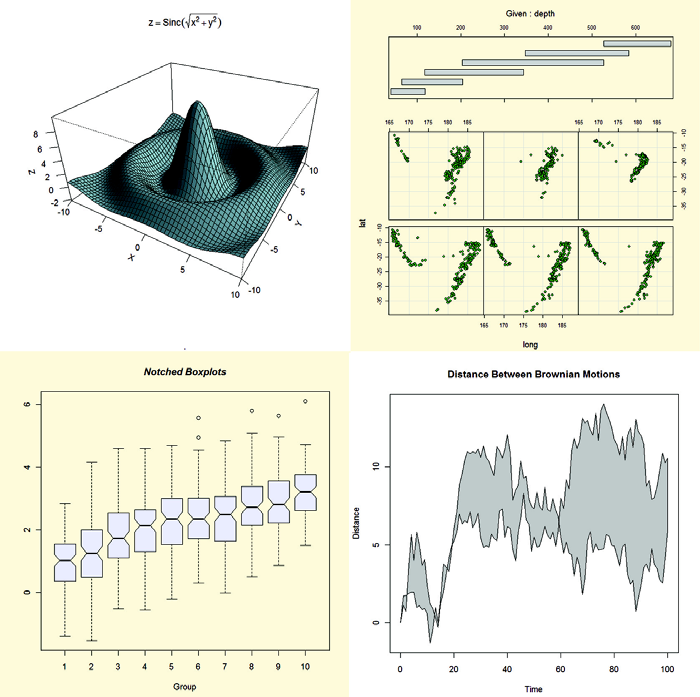
\includegraphics[width=12cm]{R_in_action_Graphs.png} \\
        {\tiny \sf Fonte: \cite{Kabacoff2015}}
      \end{center}
    \end{figure}

    A utilização da linguagem R está associado ao uso de pacotes (packages, em inglês) o que auxilia no rápido acesso e instalação do software o que facilita a utilização pela comunidade científica.\cite{Chambers2014}

    Dos diversos paradigmas de programação existentes, a linguagem R utiliza de duas delas: programação funcional e programação orientada a objetos (POO) que será abordada futuramente neste documento.\cite{Chambers2014}


  \section{áreas de Aplicação da Linguagem}
    Diversas áreas são contempladas com o uso da linguagem R. Dentre elas podemos citar as seguintes:

    \subsection{ Data Science}
      Para utilizarmos o potencial que o R tem em relação a ciência de dados, primeiro precisamos entender a sequência necessária para o trabalho com os dados descritor por \cite{HadleyWickham2017} e ilustrados em \ref{R_data_cycle}:

      \begin{enumerate}
        \item \textbf{Importar para o R}
          Não dá para utilizarmos os dados sem tê-los em mãos.
        \item \textbf{Wrangling}
          Essa etapa engloba o tratamento de dados. Ela se refere ao processo onde os dados são limpos e transformados. O termo em inglês "wrangling" significa "luta" porque você está "lutando" contra a bagunça dos dados.
        \begin{enumerate}
          \item \textit{Limpar}
            Com "limpar" quero dizer "guardar os dados de forma ordenada". Em dados organizados em planilhas, por exemplo, cada coluna representa uma variável e cada linha representa um de seus valores.
            Organizá-la ajuda a poder trabalhar com ela de forma mais consistente.
          \item \textit{Transformar}
            Nessa etapa você precisará filtrar o que de fato é relevante dentro dos dados que se tem, removendo o que não convém e se necessário, utilizando dos dados iniciais para calcular novas colunas de dados.
        \end{enumerate}
        \item \textbf{Processo de geração de conhecimento}
          É o modo como você irá analisar e obter conhecimento a partir dos dados. Existem dois meios principais, a visualização e a modelagem. Cada um deles tem suas vantagens e desvantagens, por isso numa análise real, será necessário alternar entre eles.
        \begin{enumerate}

          \item \textit{Visualização}

            É fundamentalmente uma tarefa humana. Com uma boa visualização e análise, consegue-se obter boas informações, algumas vezes até inesperadas. Isso pode levantar novas questões ou indicar que não se está analisando os dados certos para o problema abordado. Entretanto, o fato de depender da análise humana, impede uma boa escalabilidade.
          \item \textit{Modelos}
            É fundamentalmente computacional e matemático. Um modelo bem feito é utilizado para se obter respostas diretas e precisas em relação aos dados analisados pelo modelo, entretanto, um modelo não é capaz de se questionar quando a ele próprio, pois são os programadores que definem seus parâmetros. Caso algo não tenha sido desenvolvido apropriadamente, os resultados podem não ser satisfatórios. Entretanto, o fato de depender da análise computacional e matemática, permite uma boa escalabilidade.
        \end{enumerate}
      %          \item \textbf{4. Comunicação}
      %################################
      %Preencher a parte de comunicação
      %################################

      \end{enumerate}

      \begin{figure}[H]
        \begin{center}
          \caption{Fluxo dos dado} \label{R_data_cycle}
          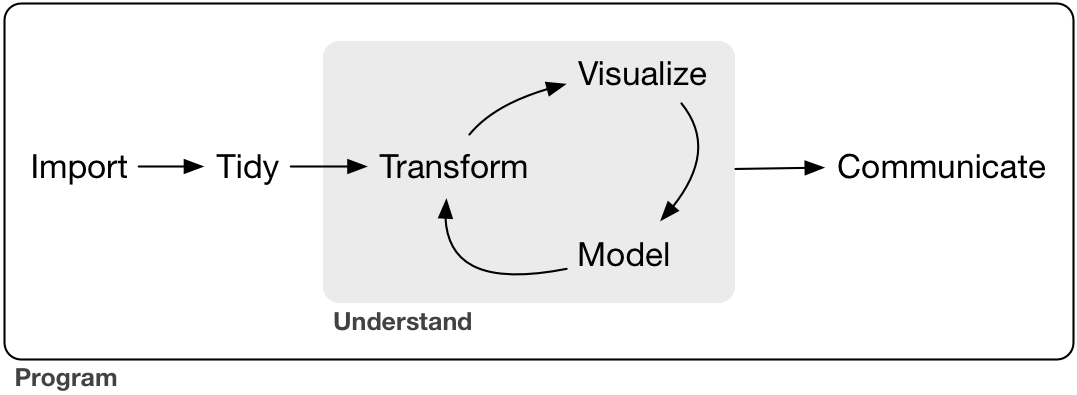
\includegraphics[width=12cm]{R_for_data_science_data_cycle.png} \\
          {\tiny \sf Fonte: \cite{HadleyWickham2017} }
        \end{center}
      \end{figure}

    \subsection{ Paradigmas}

      Como dito por \cite{Chambers2014} As evoluções na linguagem a levaram a ter suas próprias versões de programação funcional e orientada a objetos. O objetivo da evolução não foi o design em si, mas sim prover as ferramentas necessárias para pesquisa e análise de dados pela comunidade na época.Ela começou com a reprodução de funcionalidades da linguagem S, onde eram utilizados bibliotecas estatísticas, principalmente em Fortran.

      \begin{comment}
        In the case of functional programming, the realization in R is only partial, reflecting the language’s origins as well as practical considerations. In the case of OOP, there are now at least three realizations of the ideas in R, using two different paradigms. All three have significant applications and practical value. Despite all these devilish details, the main ideas remain visible and useful, particularly when programming serious applications using the language.
      \end{comment}

      Para entender essas questões computacionais em R, dois slogans podem ajudar:
      \begin{itemize}
        \item Tudo que existe é um objeto.
        \item Tudo que acontece é a chamada de uma função.
      \end{itemize}

      \subsubsection{ Orientação a objetos}

        Segundo \cite{Chambers2014} os ideis de POO em R são bem simples e intuitivas:
        \begin{enumerate}
          \item Tudo que utilizamos é um objeto e objetos devem ser estruturados para cumprir os objetivos do nosso uso.
          \item Para isso utilizaremos das relações entre diversas classes e objetos contendo atributos que interagem entre si.
          \item Uma classe pode herdar (conter) uma superclasse. Assim, seu objeto também será um objeto da superclasse.
          \item Para trabalharmos com objetos, podemos definir métodos para certas classes.
        \end{enumerate}

        Afinal, R é uma linguagem orientada a objetos? Não completamente, mas dispõe de softwares que refletem os mesmos conceitos.
        Porém, por ser uma linguagem principalmente funcional, acaba permitindo que suas definições de classe e objeto sejam feitas de diversas formas diferentes, isto faz com que acabe havendo certa confusão quanto a isso.

        Por exemplo: em R, os métodos pertencem às funções e não aos objetos em si. Por causa dessa e outras especificidades da linguagem, podemos chamá-la de uma linguagem funcional orientada a objetos, já que para ser verdadeiramente orientada a objetos, seus métodos precisariam estar encapsulados nos objetos.

        \begin{comment}
          Some of the confusion arises from not recognizing that the final item in the list above can be implemented in radically different ways, depending on the
          general paradigm of the programming language. A
          key distinction is whether the methods are to be
          embedded in some form of functional programming.
          Traditionally, most languages adopting the OOP
          %paradigm are not functional; either the language be-
          gan with objects and classes as a central motivation
          (SIMULA, Java) or added the paradigm to an exist-
          ing non-functional language (C++, Python). In such
          languages, methods were naturally associated with
          classes, essentially as callable properties of the ob-
          jects. The language would then include syntax to
          call or invoke a method on a particular object, most
          often using the infix operator “.”. The class defini-
          tion then encapsulates all the software for the class.
          Where methods are needed for other computations,
          such as special method names in Python or opera-
          tor overloading in C++, these are provided by ad-
          hoc mechanisms in the language, but the method
          remains part of the class definition.
          In a language that is functional or that aspires to
          behave functionally as S and R do, the natural role
          of methods corresponds to the intuitive meaning of
          “method”—a technique for computing the desired
          result of a function call. In functional OOP, the par-
          ticular computational technique is chosen because
          one or more arguments are objects from recognized
          classes.
          Methods in this situation belong to functions, not
          to classes; the functions are generic. In the simplest
          and most common case, referred to as a standard
          generic function in R, the function defines the formal
          arguments but otherwise consists of nothing but a
          table of the corresponding methods plus a command
          to select the method in the table that matches the
          classes of the arguments. The selected method is a
          function; the call to the generic is then evaluated as
          a call to the selected method.
          We will refer to this form of object-oriented pro-
          gramming as functional OOP as opposed to the encapsulated
          form in which methods are part of the
          class definition.
        \end{comment}

      \subsubsection{ Programação Funcional}
        Seguindo as ideias propostas por \cite{Chambers2014} a programação funcional tem princípios que nos ajudam no desenvolvimento confiável de funções para diferentes modelos, já a POO auxilia com as ferramentas necessárias para se definir o modelo devidamente.

        Veremos agora alguns princípios da programação funcional resumidamente:

        \begin{enumerate}
          \item A programação depende amplamente da definição de funções
          \item Uma função retorna um valor único de acordo com os valores passados a ela.
          \item A chamada de uma função não causa efeitos colaterais em outros cálculos.
        \end{enumerate}

        Linguagens verdadeiramente funcionais se conformam a estas ideias, tanto pelo que dispõem quanto pelo que não dispõem. Nesse sentido, R é uma linguagem funcional? Não. A sua estrutura não reforça a funcionalidade. Sua estrutura poderia ser reescrita para comportar plenamente a funcionalidade, mas isso precisaria modificar também algumas questões da linguagem que já foram bem analisadas, como por exemplo a geração de números aleatórios que é baseado no uso de estados.

        Apesar de suas limitações, a linguagem funcional permanece sendo de extrema importância para a programação estatística, como pode ser exemplificado pelos modelos estatísticos de dados frequentemente desenvolvidos em R e analisados através de uma perspectiva funcional.

        \begin{comment}
          Is R a functional programming language in this
          sense? No. The structure of the language does
          not enforce functionality; Section 2.3 examines that
          structure as it relates to functional programming
          and OOP. The evolution of R from earlier work in
          statistical computing also inevitably left portions of
          earlier pre-functional computations; Section 3 out-
          lines the history. Random number generation, for ex-
          ample, is implemented in a distinctly “state-based”
          model in which an object in the global environ-
          ment (.Random.seed) represents the current state
          of the generators. Purely functional languages have
          developed techniques for many of these computa-
          tions, but rewriting R to eliminate its huge body of
          supporting software is not a practical prospect and
          would require replacing some very well-tested and
          well-analyzed computations (random number gen-
          eration being a good example).
          Functional programming remains an important

          paradigm for statistical computing in spite of these
          limitations. Statistical models for data, the motivat-
          ing example for many features in S and R, illustrate
          the value of analyzing the software from a functional
          programming perspective. Software for fitting mod-
          els to data remains one of the most active uses of
          R. The functional validity of such software is im-
          portant both for theoretical justification and to de-
          fend the results in areas of controversy: Can we show
          that the fitted models are well-defined functions of
          the data, perhaps with other inputs to the model
          such as prior distributions considered as additional
          arguments? The structure of R as described in Sec-
          tion 2.3 can provide support for analyzing functional
          validity. Equally usefully, such analysis can also illu-
          minate the limits of functional validity for particular
          software, such as that for model-fitting.
        \end{comment}

\chapterimage{capitulo.jpg} % Chapter heading image
% Prof. Dr. Ausberto S. Castro Vera
% UENF - CCT - LCMAT - Curso de Ci\^{e}ncia da Computa\c{c}\~{a}o
% Campos, RJ,  2020
% Disciplina: Paradigmas de Linguagens de Programa\c{c}\~{a}o
% Aluno:


\chapter{ Conceitos b\'{a}sicos da Linguagem R}

Os livros b\'{a}sicos para o estudo da Linguagem R s\~{a}o: \cite{Cotton2013}, \cite{Kabacoff2015}, \cite{Wickham2016}, e \cite{Lander2014}

Neste cap\'{\i}tulo \'{e} apresentado ....

Segundo \cite{Sebesta2018}, a linguagem R,  . . .

De acordo com \cite{Sebesta2018} e \cite{roy04}, a linguagem R . . .

\cite{Sebesta2018} afirma que a linguagem R . . .

Considerando que a linguagem R (\cite{Sebesta2018}, \cite{wat90}) \'{e} considerada como ....

    %%%%%%%%=================================
    \section{Vari\'{a}veis e constantes}
    %%%%%%%%=================================


    %%%%%%%%=================================
    \section{Tipos de Dados B\'{a}sicos}
    %%%%%%%%=================================

     %%%%%%%%=================================
    \section{Tipos de Dados de Cole\c{c}\~{a}o}
    %%%%%%%%=================================

     %%%%%%%%=================================
    \section{Opera\c{c}\~{o}es L\'{o}gicas}
    %%%%%%%%=================================



    %%%%%%%%=================================
    \section{Estrutura de Controle e Fun\c{c}\~{o}es}
    %%%%%%%%=================================



    %%%%%%%%======================
    \section{M\'{o}dulos}
    %%%%%%%%======================



    %%%%%%%%======================
    \section{Orienta\c{c}\~{a}o a Objetos}
    %%%%%%%%======================



\chapter{Aplicações da Linguagem R}
  \begin{comment} //Cabeçalho
    Prof. Dr. Ausberto S. Castro Vera
    UENF - CCT - LCMAT - Curso de Ciência da Computação
    Campos, RJ,  2021
    Disciplina: Paradigmas de Linguagens de Programação
  \end{comment}
  \begin{comment} //Comentários iniciais
    Devem ser mostradas pelo menos CINCO aplicações completas da linguagem, e em cada caso deve ser apresentado:
    \begin{itemize}
      \item Uma breve descrição da aplicação,
      \item O código completo da aplicação,
      \item Imagens do código fonte no compilador-interpretador,
      \item Imagens dos resultados após a compilação-interpretação do código fonte
      \item Links e referências bibliográficas de onde foi obtido a aplicação
    \end{itemize}
  \end{comment}
  \section{Operações básicas}
  	\begin{itemize}
  		\item \textbf{Descrição}
  		
  		  O código abaixo mostrará os seguintes conceitos básicos presentes em linguagens de programação:
  		  \begin{enumerate}
  			\item Comentários
  			\item Imprimir informações
  			\item Fazer operações com variáveis
  			\item Obter dados pela entrada padrão
  			\item Operações Lógicas
  			\item Estruturas de controle de fluxo
  			\item Funções
  		\end{enumerate}
  		  Mais abaixo é mostrada a Figura \ref{Codigo_1} que apresenta a execução do código no ambiente de desenvolvimento RStudio.
  	
  		\item \textbf{Código}
  		\color{blue}
  		\verbatiminput{1-Operacoes_Basicas.r}
  		\color{black}
  		
  		  %\begin{lstlisting}[language=R]
  		  %\end{lstlisting}
  		  
  		\item \textbf{Imagens do código com resultados}
  		  \begin{figure}[H]  \label{Codigo_1}
  		  	\centering
  		  		\caption{Operações básicas no RStudio}
  		  		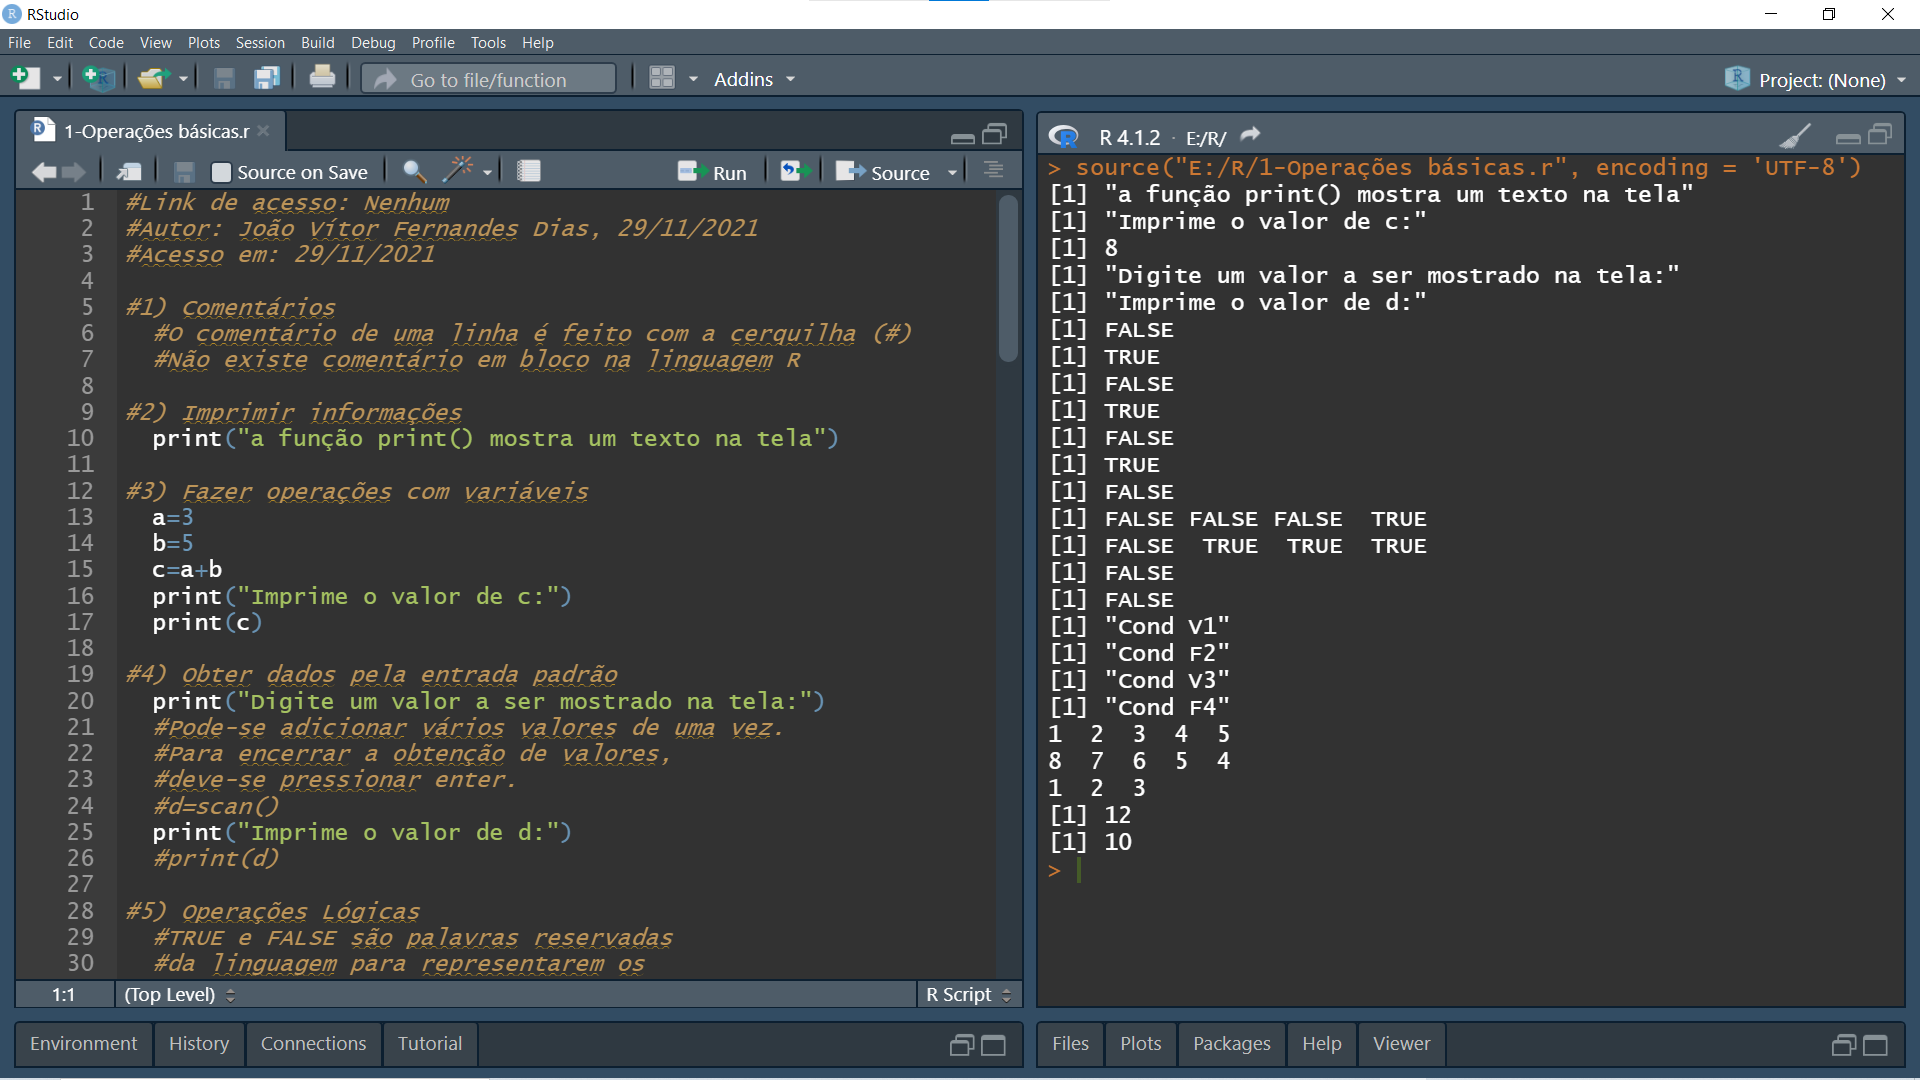
\includegraphics[width=16cm]{PicturesJoaoDias/Codigos/Codigo1.png}
  		  		{\tiny \sf Fonte: autoria própria}
  		  \end{figure}
  		  
  		\item \textbf{Links e referências bibliográficas das aplicações}
  		\\ \\
  		  Código de autoria própria.
  		
  	\end{itemize}
  
  \section{Programas gráficos}
  \begin{itemize}
  	\item \textbf{Descrição}
  	
  	  Este programa apresenta um código de exemplo para demonstrar a capacidade de diversidade de gráficos gerados em R. O exemplo escolhido apresenta um gráfico ternário representando as cores dos pixels de acordo com a quantidade de vermelho, verde e azul.
  	  
  	  Mais abaixo é mostrada a Figura \ref{Codigo_2a} que apresenta a execução do código no ambiente de desenvolvimento RStudio.
  	  %e também a Figura \ref{Codigo_2b} que apresenta o gráfico gerado pela execução do programa.
  	  
  	  
  	\item \textbf{Código}
  	
  	
  	\color{blue}
  	\verbatiminput{2-Programas_Graficos.r}
  	\color{black}
  	
  	\item \textbf{Imagens do código com resultados}
  	
	  	\begin{figure}[H]  \label{Codigo_2a}
	  		\centering
	  		\caption{Programas gráficos no RStudio}
	  		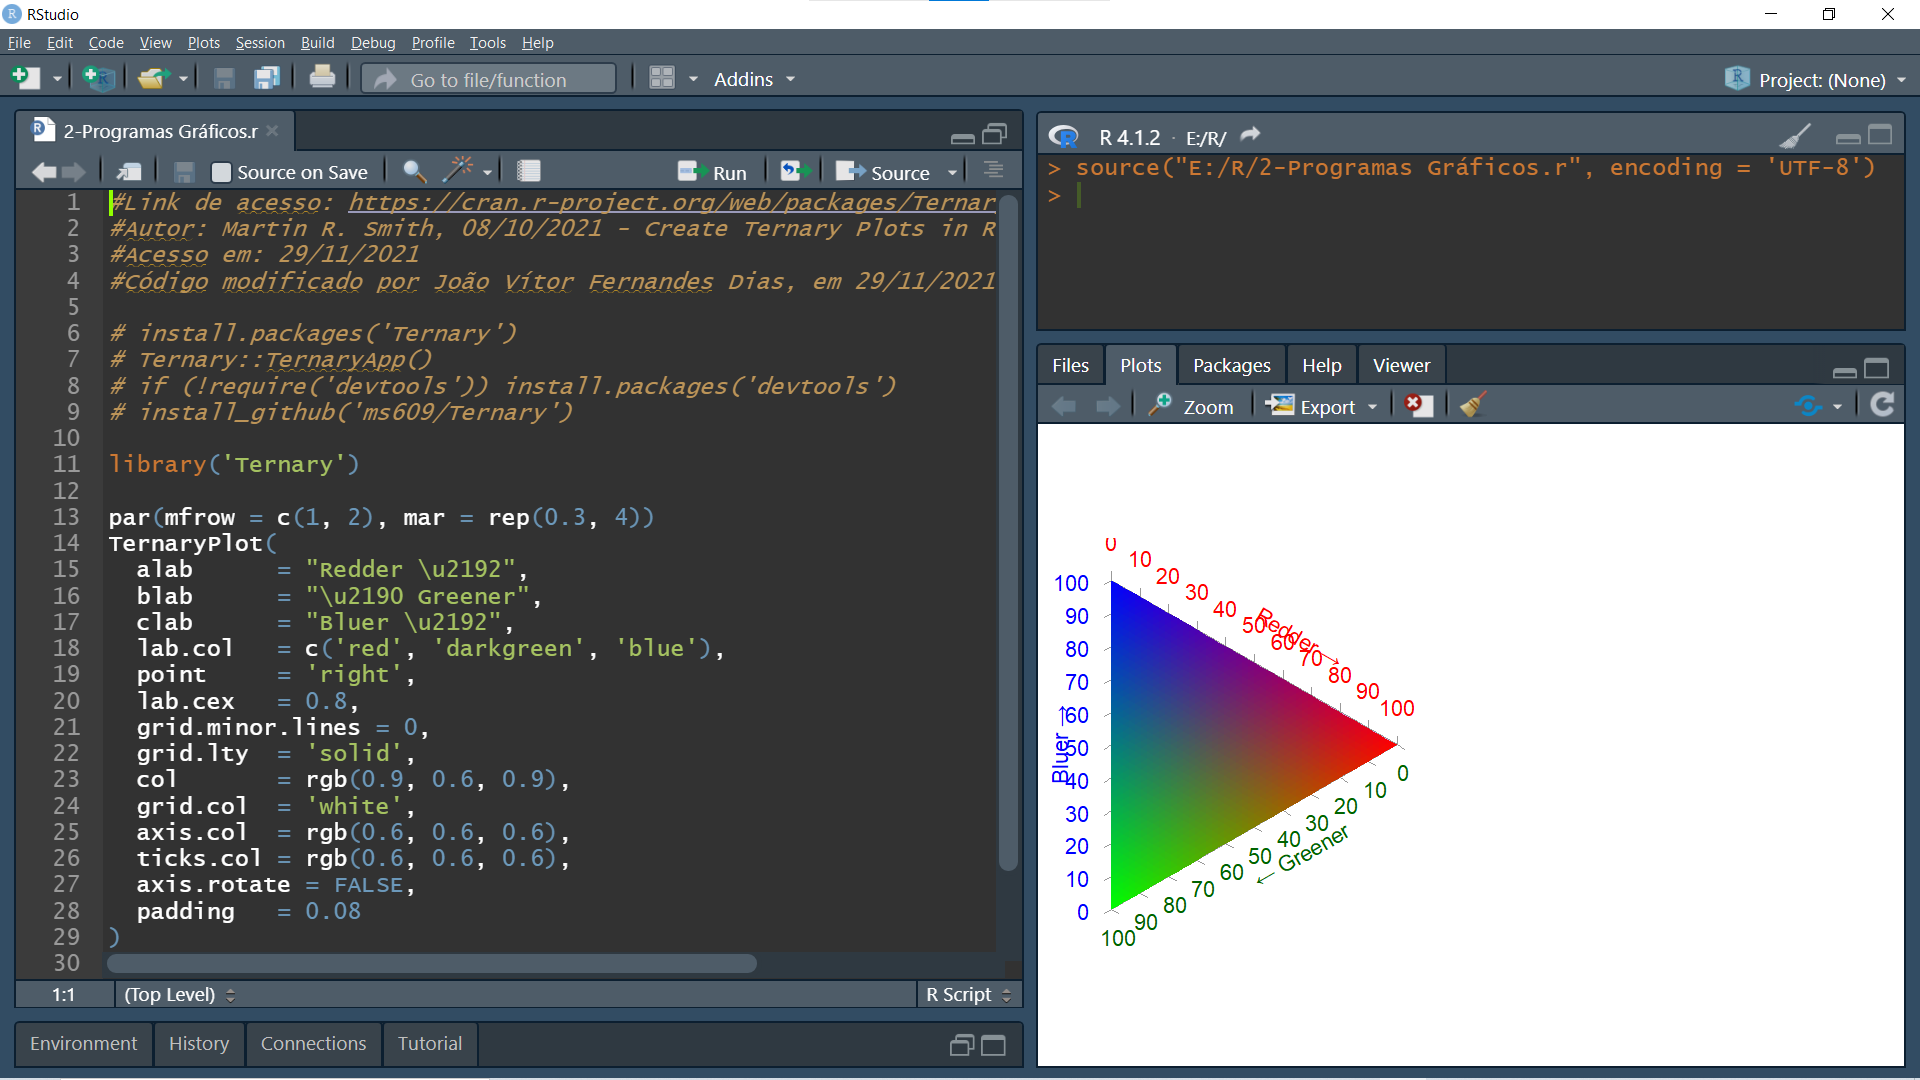
\includegraphics[width=16cm]{PicturesJoaoDias/Codigos/Codigo2a.png}
	  		{\tiny \sf Fonte: autoria própria}
	  	\end{figure}
	  	\begin{comment}	%IMAGEM SENDO REFERENCIADA DE FORMA ESTRANHA
	  		
	  	\begin{figure}[H]  \label{Codigo_2b}
	  		\centering
	  		\caption{Gráfico resultante}
	  		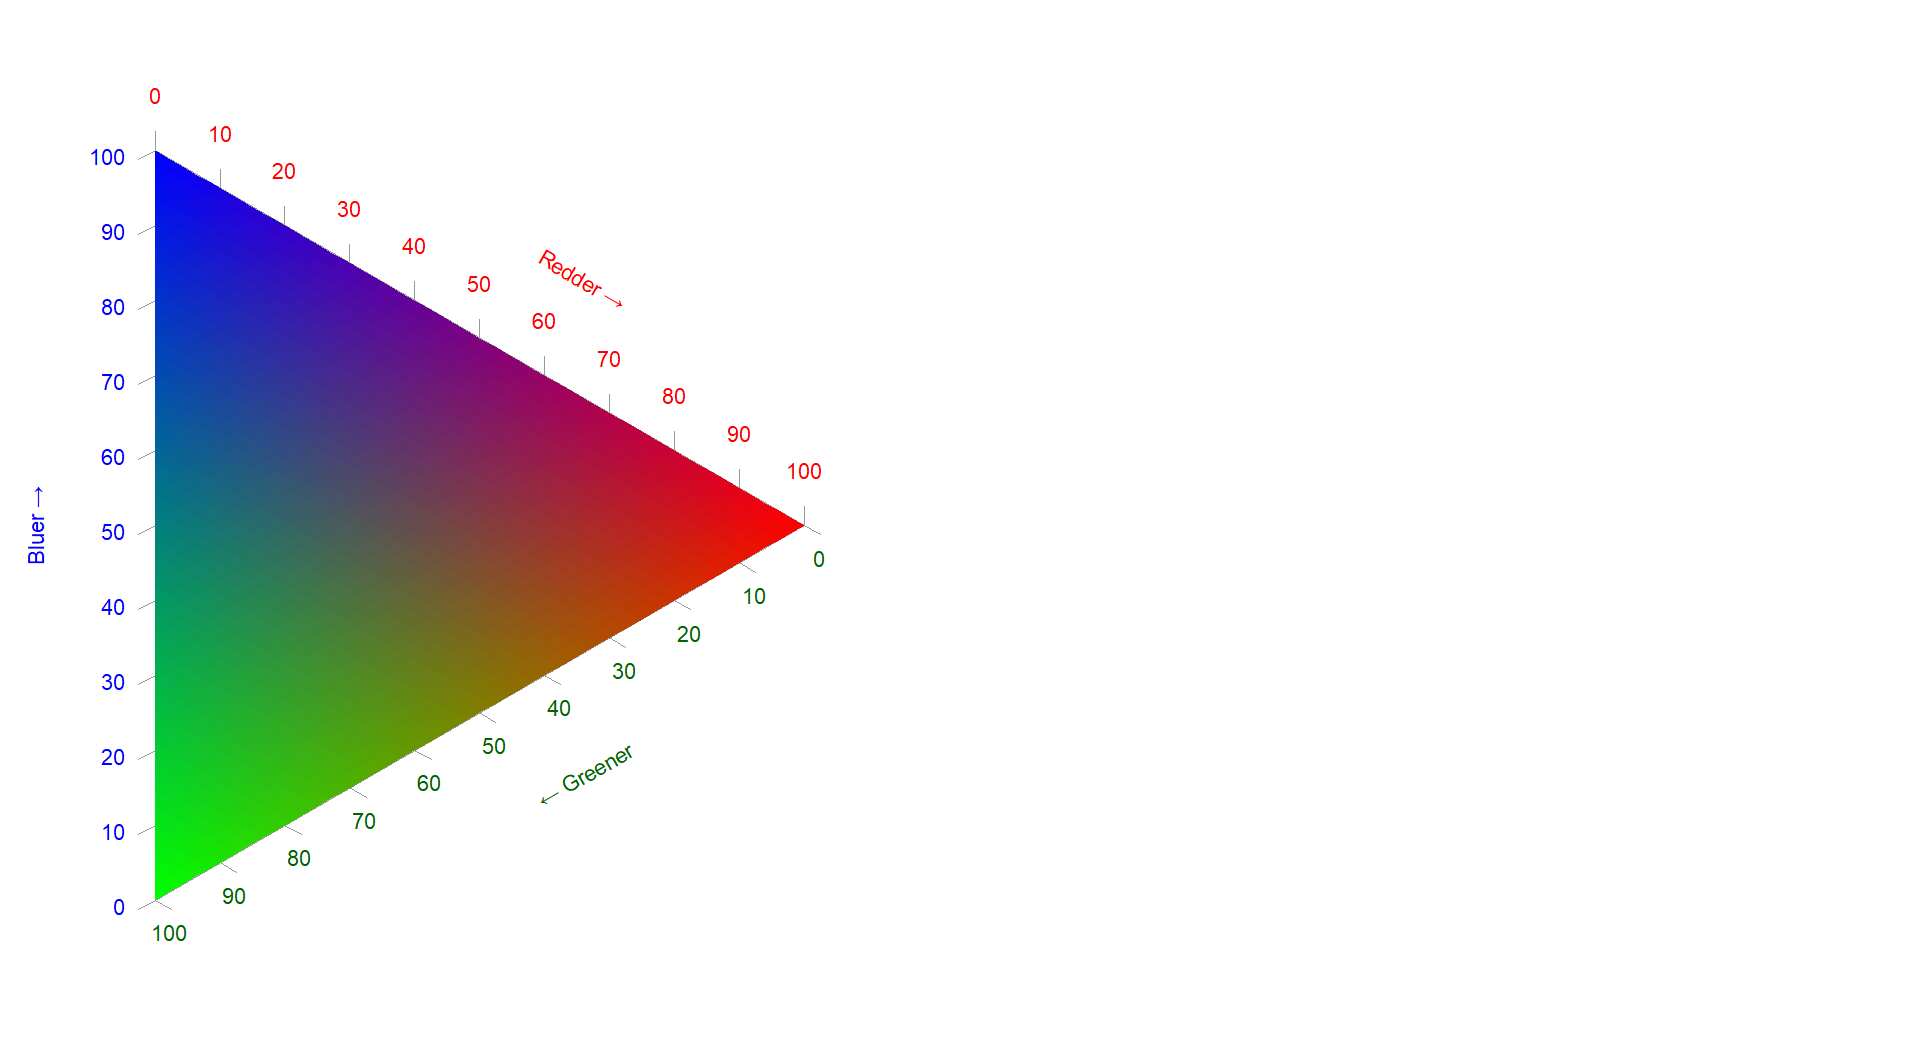
\includegraphics[width=16cm]{PicturesJoaoDias/Codigos/Codigo2b.png}
	  		{\tiny \sf Fonte: autoria própria}
	  	\end{figure}
  	
        \end{comment}
    
  	\item \textbf{Links e referências bibliográficas das aplicações}
  	  \\ \\
  	  \textit{Link referente ao código:} 
  	  \href{https://cran.r-project.org/web/packages/Ternary/vignettes/Ternary.html}{Create Ternary Plots in R}
  	
  	  \textit{Desenvolvido por:} Martin R. Smith, 08/10/2021
  	
  	  \textit{Acesso em:} 29/11/2021
  	
  \end{itemize}
  \section{Programas com Objetos}
  \begin{itemize}
  	\item \textbf{Descrição}
  	
  	  O código seguinte apresenta alguns exemplos de estruturas para criação de objetos e classes, utilizando a linguagem R. No código abaixo é criado um objeto endereço e também duas classes, uma classe S3 representando um cachorro, e uma classe S4 representando uma caneta.
  	  
  	  Mais abaixo é mostrada a Figura \ref{Codigo_3} que apresenta a execução do código no ambiente de desenvolvimento RStudio.
  	
  	\item \textbf{Código} 
  	
  	\color{blue}
  	\verbatiminput{3-Objetos.r}
  	\color{black}
  	
  	\item \textbf{Imagens do código com resultados}
	  	
	  	\begin{figure}[H]  \label{Codigo_3}
	  		\centering
	  		\caption{Programas com objetos no RStudio}
	  		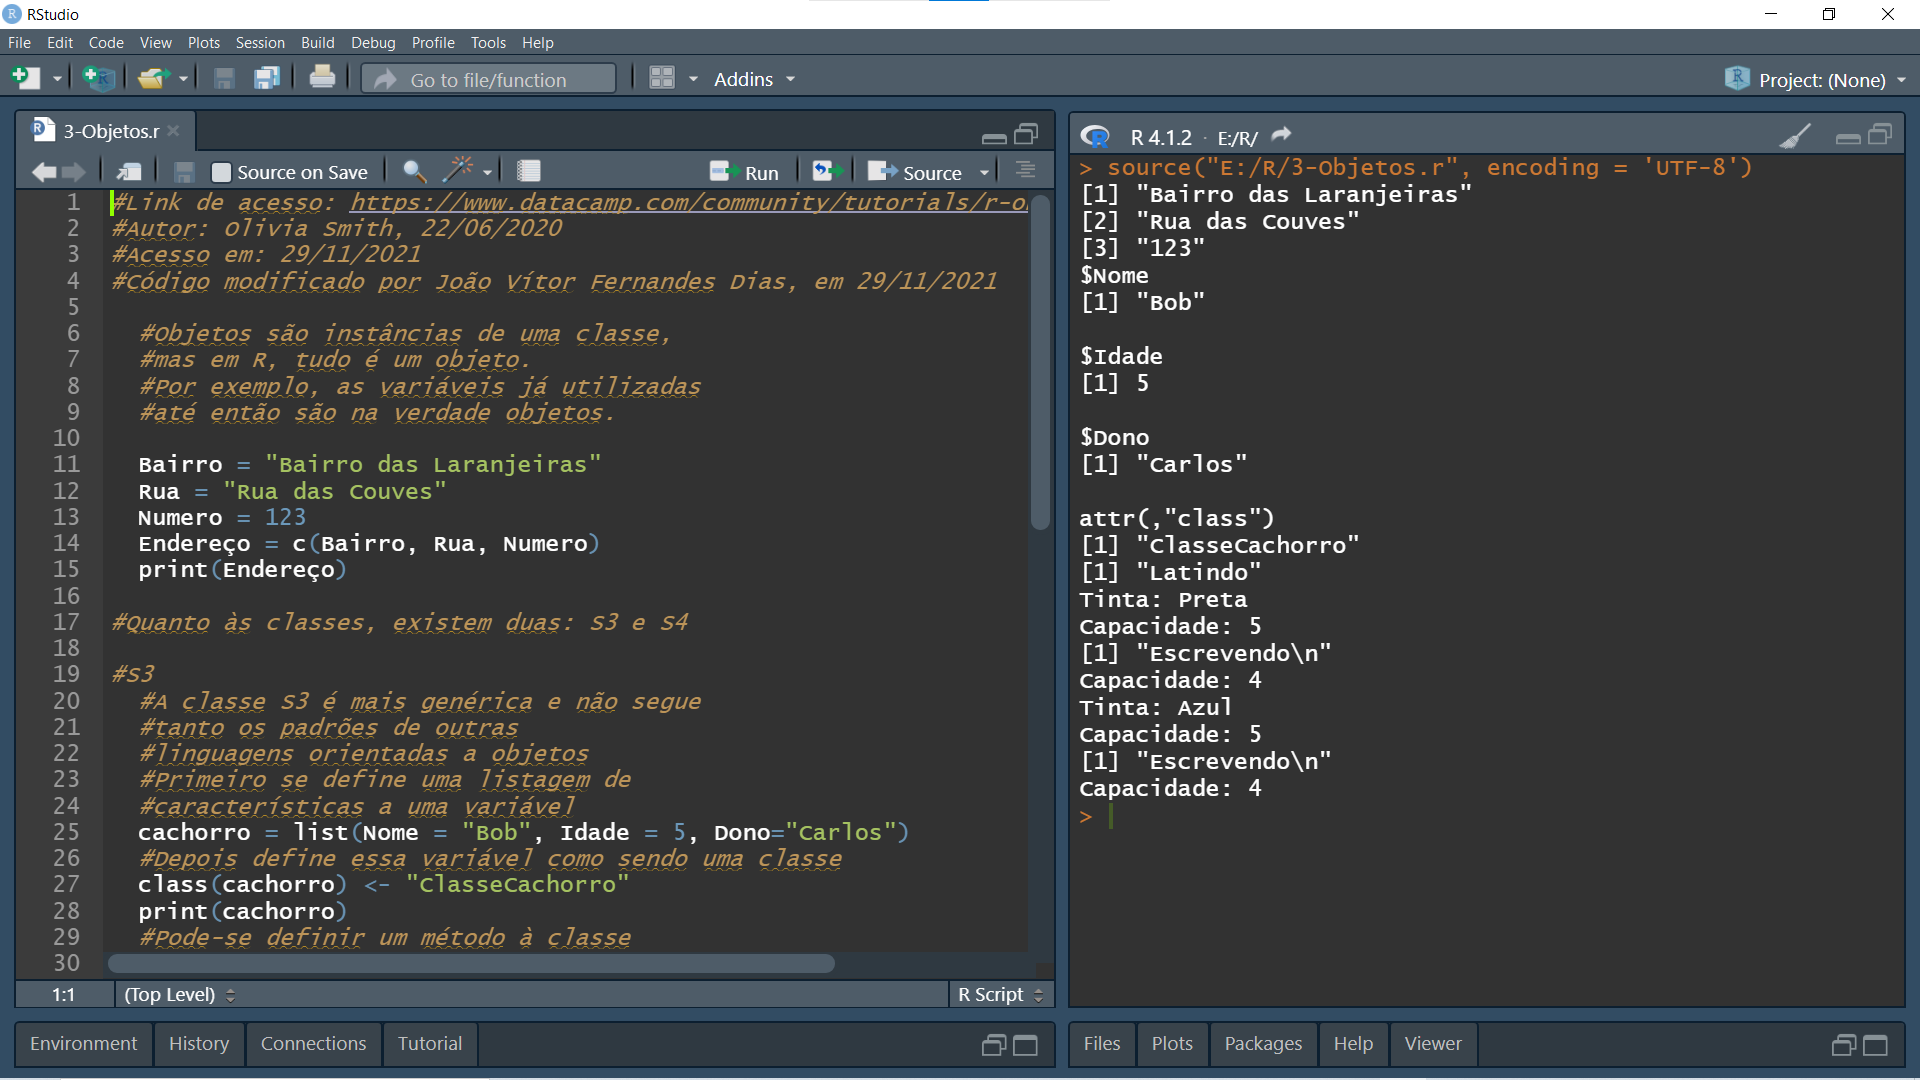
\includegraphics[width=16cm]{PicturesJoaoDias/Codigos/Codigo3.png}
	  		{\tiny \sf Fonte: autoria própria}
	  	\end{figure}
  	
  	\item \textbf{Links e referências bibliográficas das aplicações}
  	  \\ \\
  	  \textit{Link referente ao código:} 
  	  \href{https://www.datacamp.com/community/tutorials/r-objects-and-classes}{R objects and classes}
  	
  	  \textit{Desenvolvido por:} Olivia Smith, 22/06/2020
  	
  	  \textit{Acesso em:} 29/11/2021
  	
  \end{itemize}
	
  \section{O algoritmo Quicksort - Implementação}
  \begin{itemize}
  	\item \textbf{Descrição}
  	  
  	  O código abaixo apresenta uma forma recursiva do conhecido algoritmo de Quicksort, onde ele recursivamente seleciona um elemento pivô e separa o vetor entre elementos maiores e menores que ele, até que reste apenas um elemento a ser comparado, então retorna os valores e obtém-se o vetor ordenado.
  	
  	  Mais abaixo é mostrada a Figura \ref{Codigo_4} que representa a execução do código no ambiente de desenvolvimento RStudio Cloud.
  	
  	\item \textbf{Código}
  	
  	\color{blue}
  	\verbatiminput{4-QuickSort.r}
  	\color{black}
  	
  	\item \textbf{O algoritmo Quicksort no RStudio Cloud}
  	
      \begin{figure}[H]  \label{Codigo_4}
        \centering
        \caption{O algoritmo Quicksort no RStudio Cloud}
        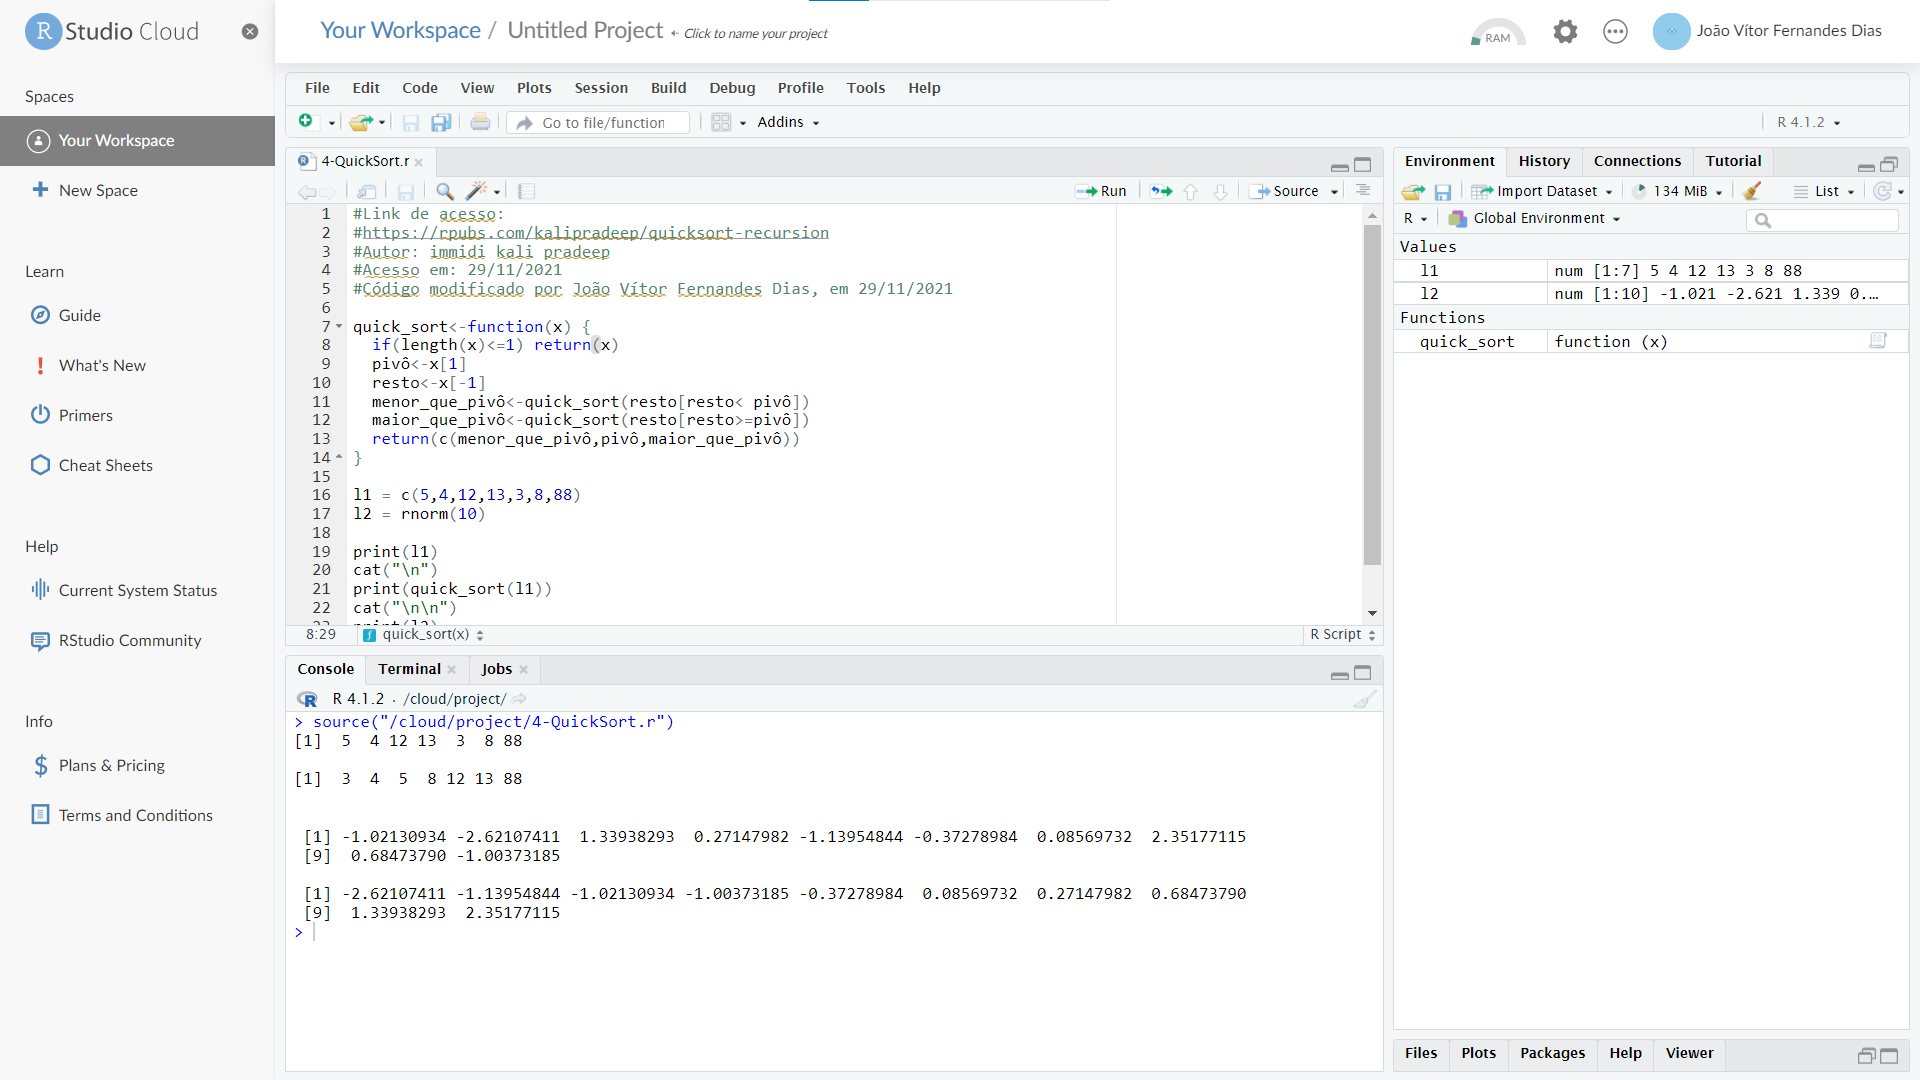
\includegraphics[width=16cm]{PicturesJoaoDias/Codigos/Codigo4_cloud.png}
        {\tiny \sf Fonte: autoria própria}
      \end{figure}
  	
  	\item \textbf{Links e referências bibliográficas das aplicações}
  	\\ \\
  	\textit{Link referente ao código:} 
  	\href{https://rpubs.com/kalipradeep/quicksort-recursion}{Quicksort Recursion}
  	
  	\textit{Desenvolvido por:} Immidi Kali Pradeep
  	
  	\textit{Acesso em:} 29/11/2021
  	
  \end{itemize}
	
  \section{Aplicações com Banco de Dados}
  \begin{itemize}
  	\item \textbf{Descrição}
  	
  	  O código abaixo apresenta duas formas de se lidar com um banco de dados. A primeira é mais simples e lida com dados inseridos manualmente em um data set. A segunda é mais avançada e próxima do uso geral de dados, que é utilizando um arquivo csv. No primeiro exemplo são listadas algumas pessoas e suas respectivas idades. No segundo exemplo é demonstrado o uso de dados estruturados referentes ao salário mínimo dos Estados Unidos entre os anos de 1938 e 2020.
  	
  	  Mais abaixo é mostrada a Figura \ref{Codigo_5} que representa a execução do código no ambiente de desenvolvimento RStudio.
  	  
  	\item \textbf{Código} 
  	
  	
  	\color{blue}
  	\verbatiminput{5-Database.r}
  	\color{black}
  	
  	\item \textbf{Aplicações com Banco de Dados no RStudio}
  	
	  	\begin{figure}[H]  \label{Codigo_5}
	  		\centering
	  		\caption{Gráfico resultante}
	  		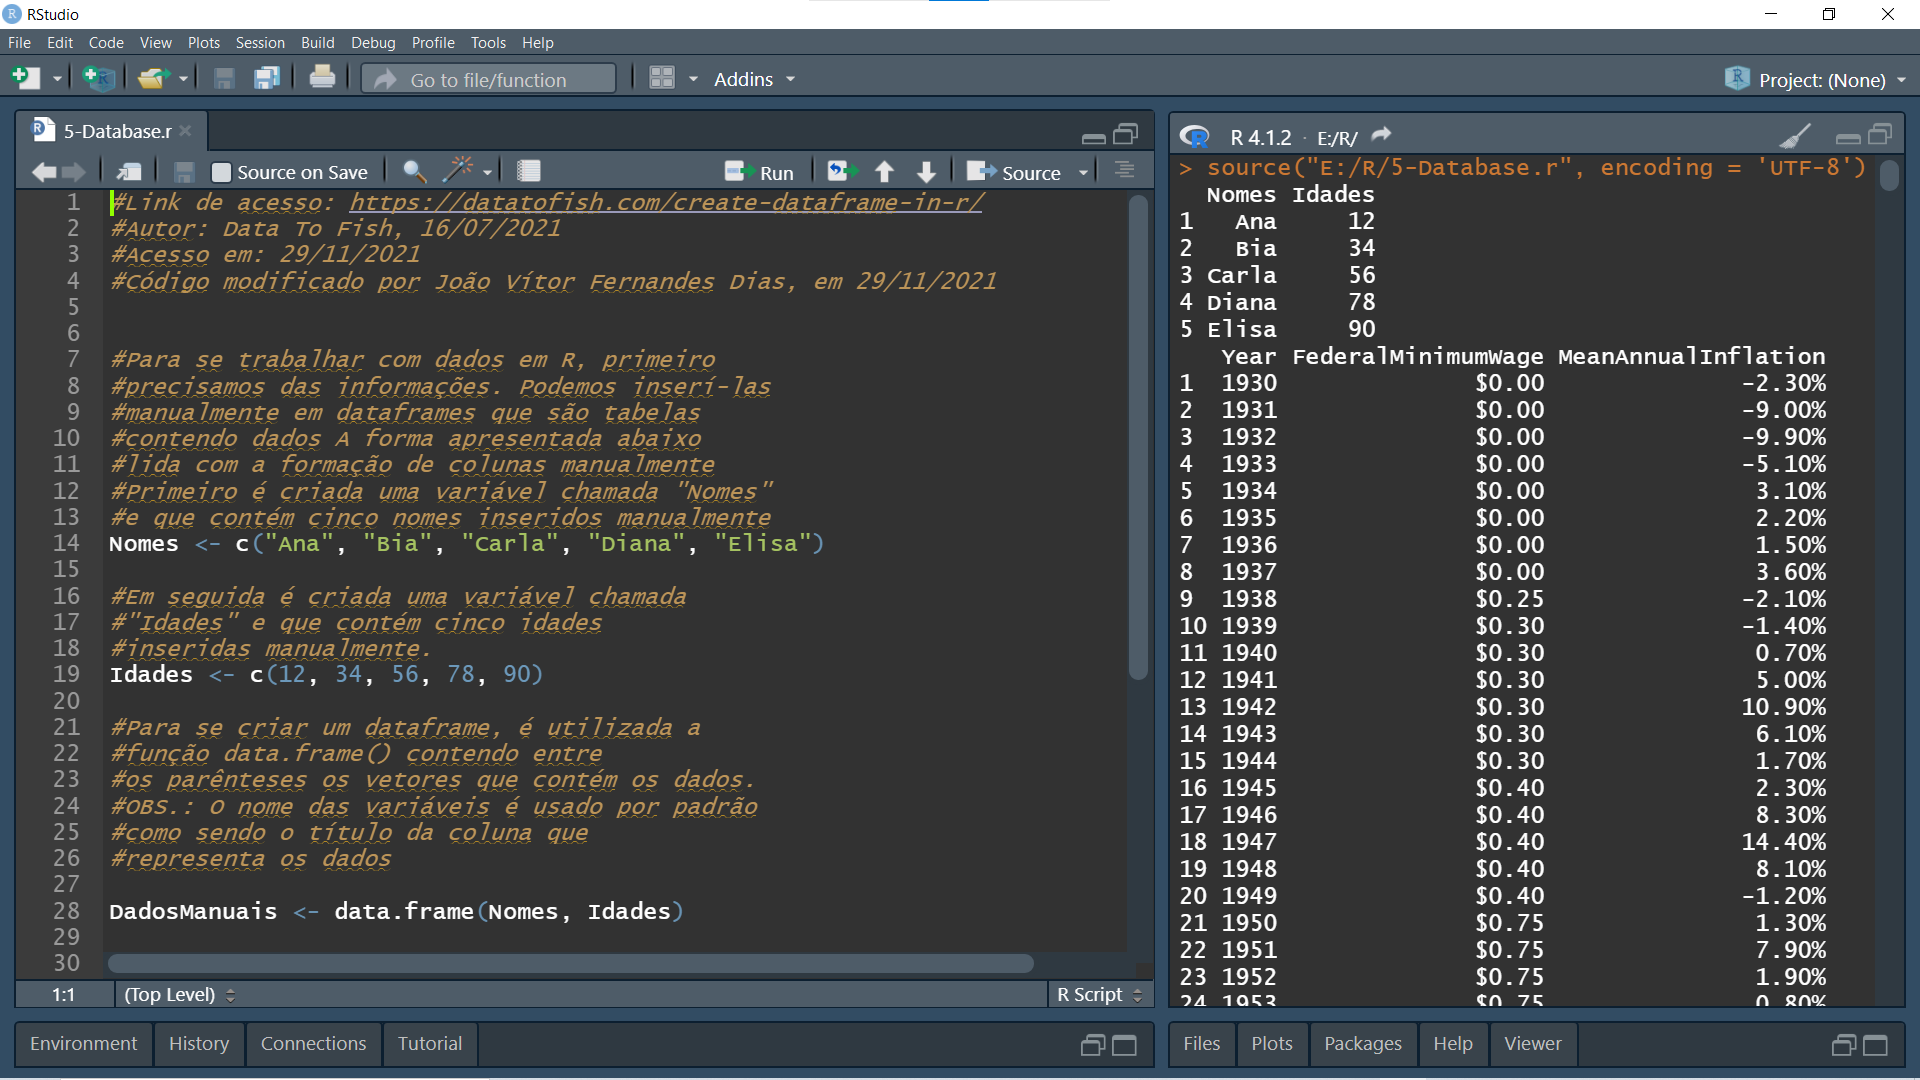
\includegraphics[width=16cm]{PicturesJoaoDias/Codigos/Codigo5.png}
	  		{\tiny \sf Fonte: autoria própria}
	  	\end{figure}
  	
  	\item \textbf{Links e referências bibliográficas das aplicações}
  	  \\ \\
  	  \textit{Link referente ao código:} 
  	  \href{https://datatofish.com/create-dataframe-in-r/}{Create  Dataframe in R}
  	  
  	  \textit{Desenvolvido por:} Data To Fish, 16/07/2021
  	  
  	  \textit{Acesso em:} 29/11/2021
  	  \\ \\
  	  \textit{Link referente ao arquivo CSV:}
  	  \href{https://www.kaggle.com/brandonconrady/us-minimum-wage-1938-2020}{US Minimum Wage 1938-2020}
  	  
  	  \textit{Desenvolvido por:} Brandon Conrady, 29/11/2021
  	  
  	  \textit{Acesso em:} 29/11/2021  	
  \end{itemize}
\chapter{Ferramentas existentes e utilizadas}
	%FALTA INSERIR AS IMAGENS DAS IDEs
  \begin{comment}
    Prof. Dr. Ausberto S. Castro Vera
    UENF - CCT - LCMAT - Curso de Ciência da Computação
    Campos, RJ,  2021
    Disciplina: Paradigmas de Linguagens de Programação
    Neste capítulo devem ser apresentadas pelo menos DUAS (e no máximo 5) ferramentas consultadas e utilizadas para realizar o trabalho, e usar nas aplicações. Considere em cada caso:
    \begin{itemize}
        \item Nome da ferramenta (compilador-interpretador)
        \item Endereço na Internet
        \item Versão atual e utilizada
        \item Descrição simples (máx 2 parágrafos)
        \item Telas capturadas da ferramenta
        \item Outras informações
    \end{itemize}
    \section{Editor MNOP}
    \section{Compilador XYZ}
    \section{Interpretador UVW}
    \section{Ambientes de Programação IDE MNP}
  \end{comment}
  Neste capítulo serão apresentadas e ilustradas algumas das ferramentas disponíveis para se utilizar a linguagem R, sendo elas o interpretador R GUI e as IDEs RStudio Desktop, RStudio Cloud, Visual Studio Code e Jupyter Notebook.
  \section{R GUI}
      \begin{itemize}
      	
      	\item \textit{Imagem da ferramenta:}
      	
      	\begin{figure}[H]  \label{RGUI}
      		\centering
      		\caption{R GUI logo após a instalação}
      		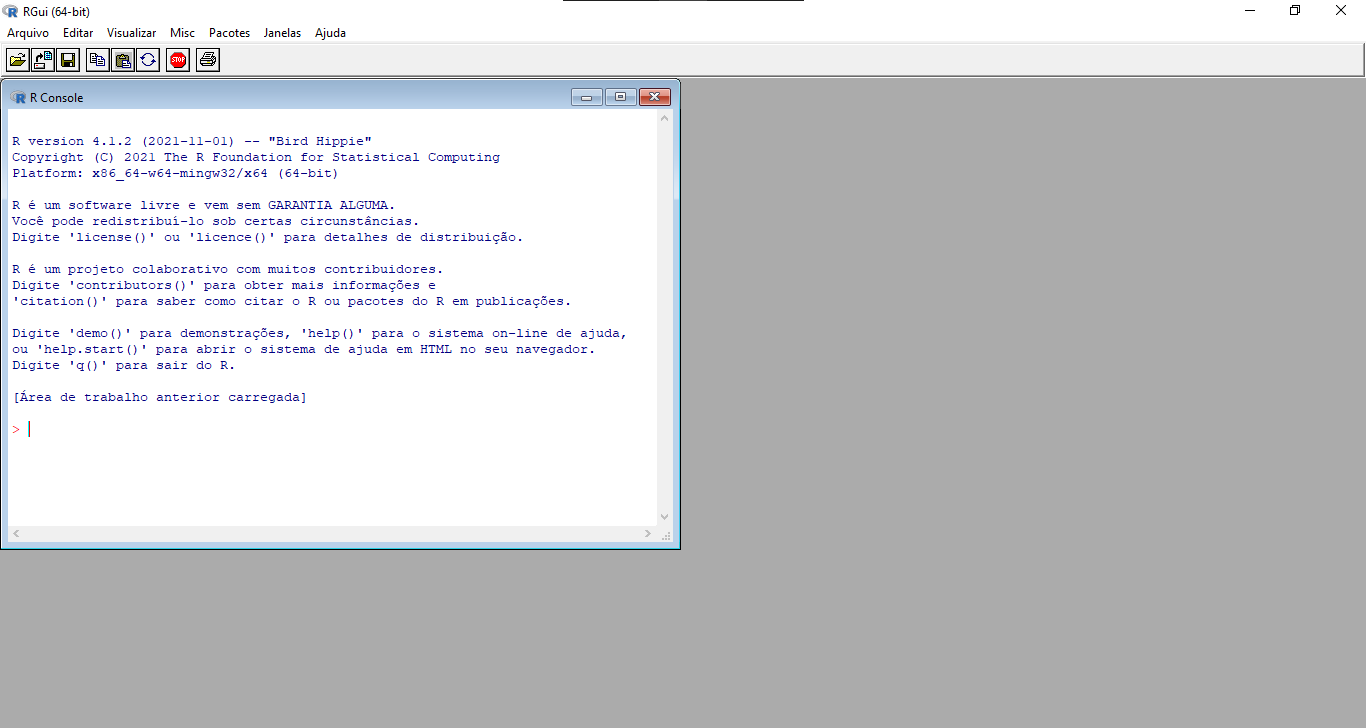
\includegraphics[width=16cm]{PicturesJoaoDias/Ferramentas/RGUI/R_GUI_tela_inicial.png}
      		{\tiny \sf Fonte: autoria própria}
      	\end{figure}
      	
          \item \textit{Link de acesso:} \href{https://cran.rstudio.com/bin/windows/base/}{R GUI} (interpretador)
          \item \textit{Versão:} 4.1.2
          \item \textit{Descrição e comentários:}
            Ferramenta padrão para executar os scripts em R, é interessante pois apresenta algumas demonstrações de coisas que podem ser feitas em R. Executar os códigos nele me pareceu pouco intuitivo. A Figura \ref{RGUI} ilustra a ferramenta logo após a sua instalação.
      \end{itemize}

\newpage
  \section{RStudio Desktop}
    \begin{itemize}
    	
    	\item \textit{Imagem da ferramenta:}
    	
    	\begin{figure}[H]  \label{RStudio_Desktop}
    		\centering
    		\caption{RStudio Desktop logo após a instalação}
    		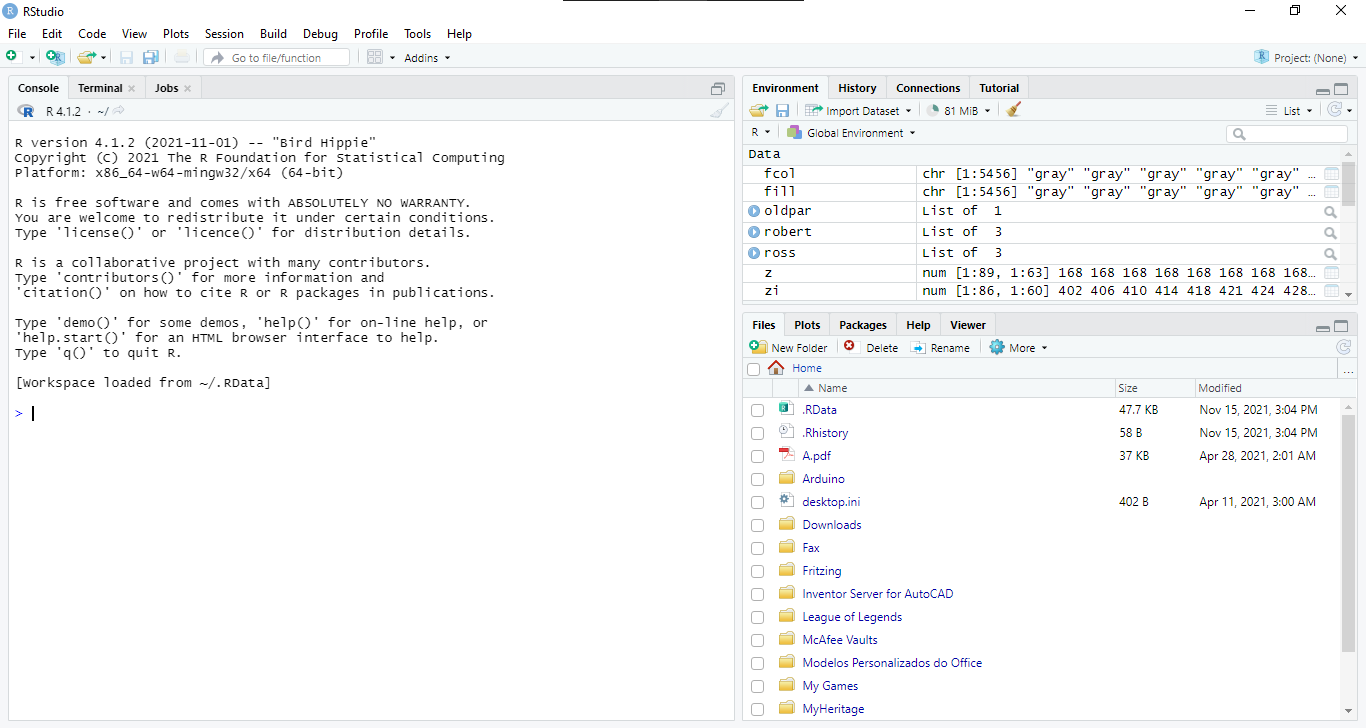
\includegraphics[width=16cm]{PicturesJoaoDias/Ferramentas/RStudio Desktop/RStudio_tela_inicial.png}
    		{\tiny \sf Fonte: autoria própria}
    	\end{figure}
    	
        \item  \textit{Link de acesso:} \href{https://www.rstudio.com/products/rstudio/download/#download}{RStudio Desktop}  (IDE)
        \item \textit{Versão:} 2021.09.1+372 "Ghost Orchid" Release for Windows
        \item \textit{Descrição e comentários:}
          IDE muito utilizada para desenvolvimento de códigos na linguagem R. Inicialmente me senti mais confortável com um ambiente mais moderno e com a possibilidade de configuração de um modo escuro. Há também uma janela que permite seguir tutoriais, o que é bom para iniciantes. Entretanto, assim como no R GUI, não senti que rodar o primeiro código tenha sido intuitivo o bastante. A Figura \ref{RStudio_Desktop} ilustra a ferramenta logo após a sua instalação.
    \end{itemize}
	\newpage
  \section{RStudio Cloud}
      \begin{itemize}
      	
      	\item \textit{Imagem da ferramenta:}
      	
      	\begin{figure}[H]  \label{RStudio_Cloud}
      		\centering
      		\caption{RStudio Cloud logo após a execução}
      		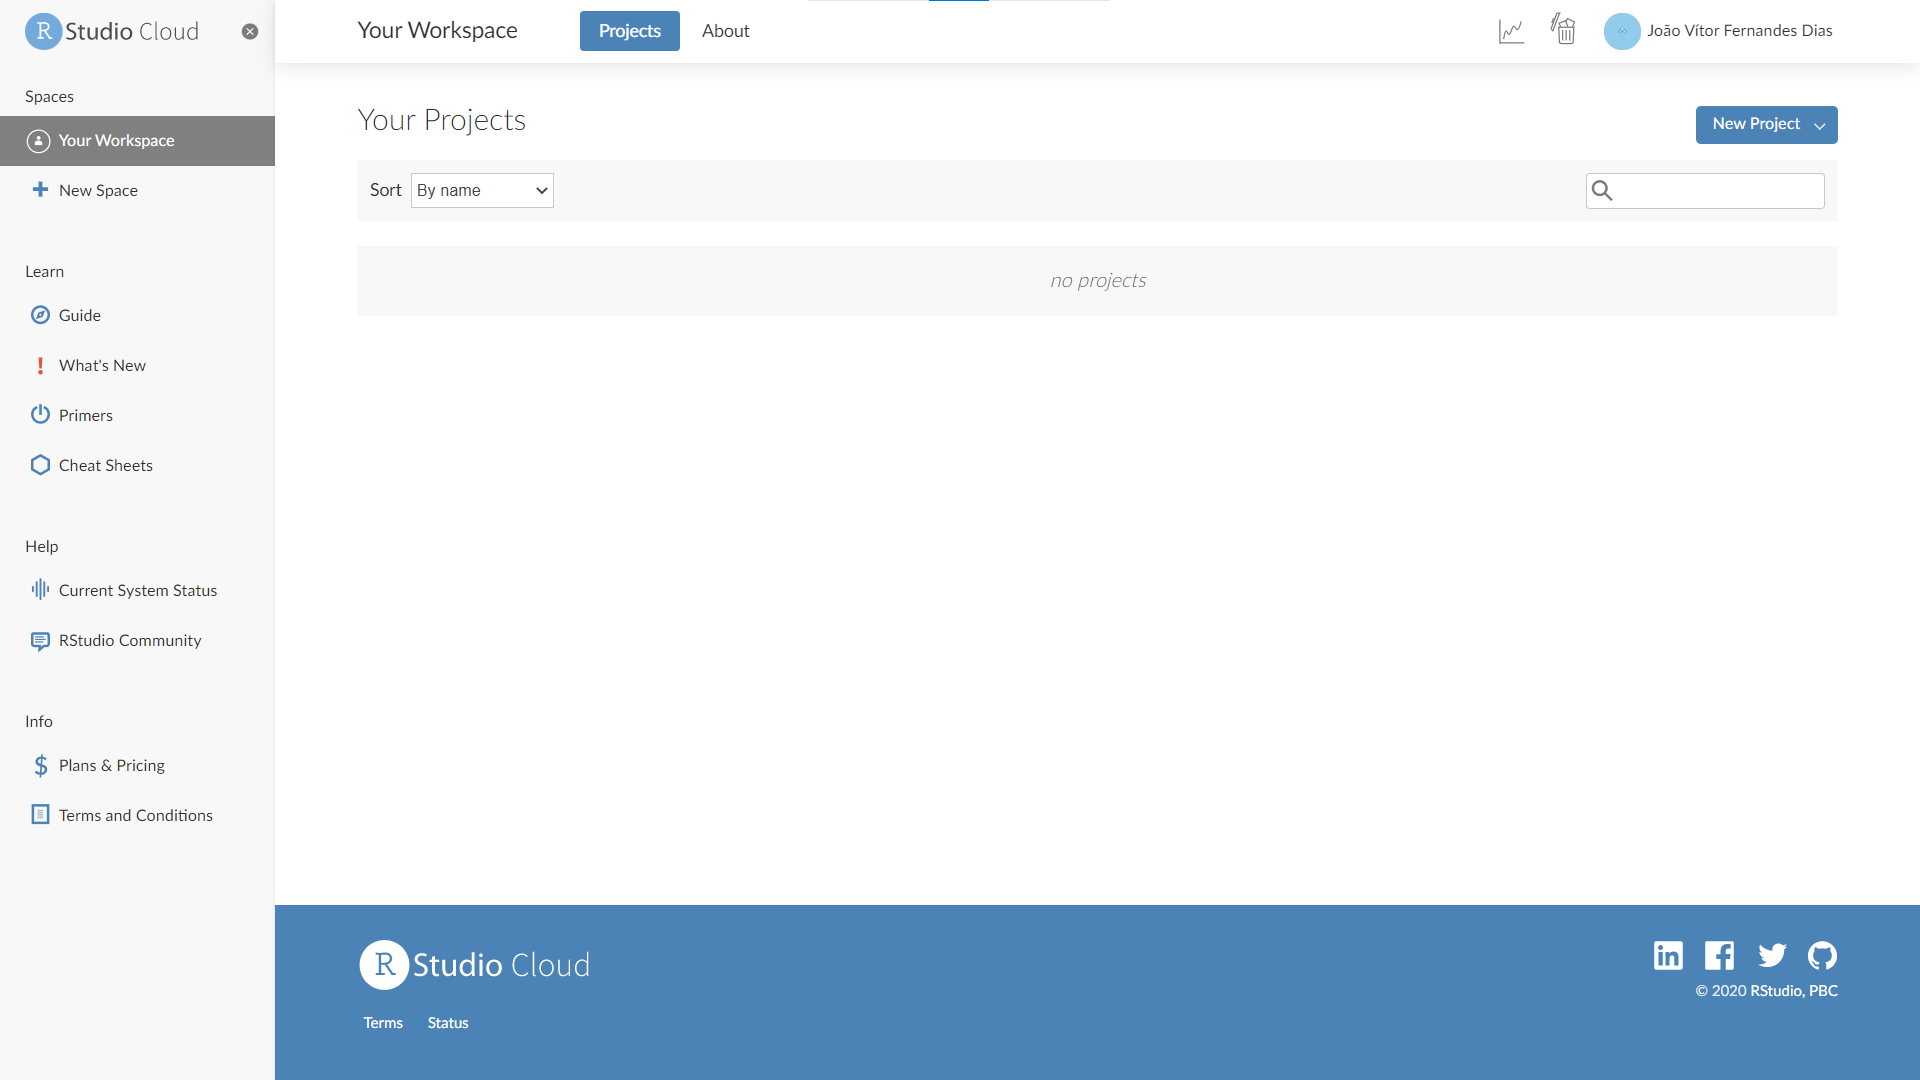
\includegraphics[width=16cm]{PicturesJoaoDias/Ferramentas/RStudio Cloud/RStudio_Cloud_Tela-Inicial.png}
      		{\tiny \sf Fonte: autoria própria}
      	\end{figure}
      	
          \item \textit{Link de acesso:} \href{https://rstudio.cloud/}{URL de acesso ao RStudio Cloud} (IDE e interpretador)
          \item \textit{Versão:} 1.4.1718-1 "Trampled Dandelion" for Ubuntu Bionic

          \item \textit{Descrição e comentários:}
          É bem similar ao RStudio Desktop, só que online e por isso tem a facilidade da portabilidade, mas tem a desvantagem da perda de conexão resultando em pausa no trabalho. Talvez por ter tido contato com o RStudio Desktop antes, a navegação pelo RStudio Cloud me pareceu mais intuitiva. Utilizando do markdown R pude executar o código de forma mais direta. Após essa descoberta no RStudio Cloud, descobri que pode-se usar o R markdown também no RStudio Desktop. Então generalizando, dá para entendermos o RStudio Cloud como sendo um "RStudio Desktop" online. A Figura \ref{RStudio_Cloud} ilustra a ferramenta logo após a sua execução.
      \end{itemize}

\newpage
  \section{Visual Studio Code}
  
  \begin{itemize}
  	
  	\item \textit{Imagem da ferramenta:}
  	
  	\begin{figure}[H]  \label{Visual_Studio_Code}
  		\centering
  		\caption{Visual Studio Code logo após a instalação}
  		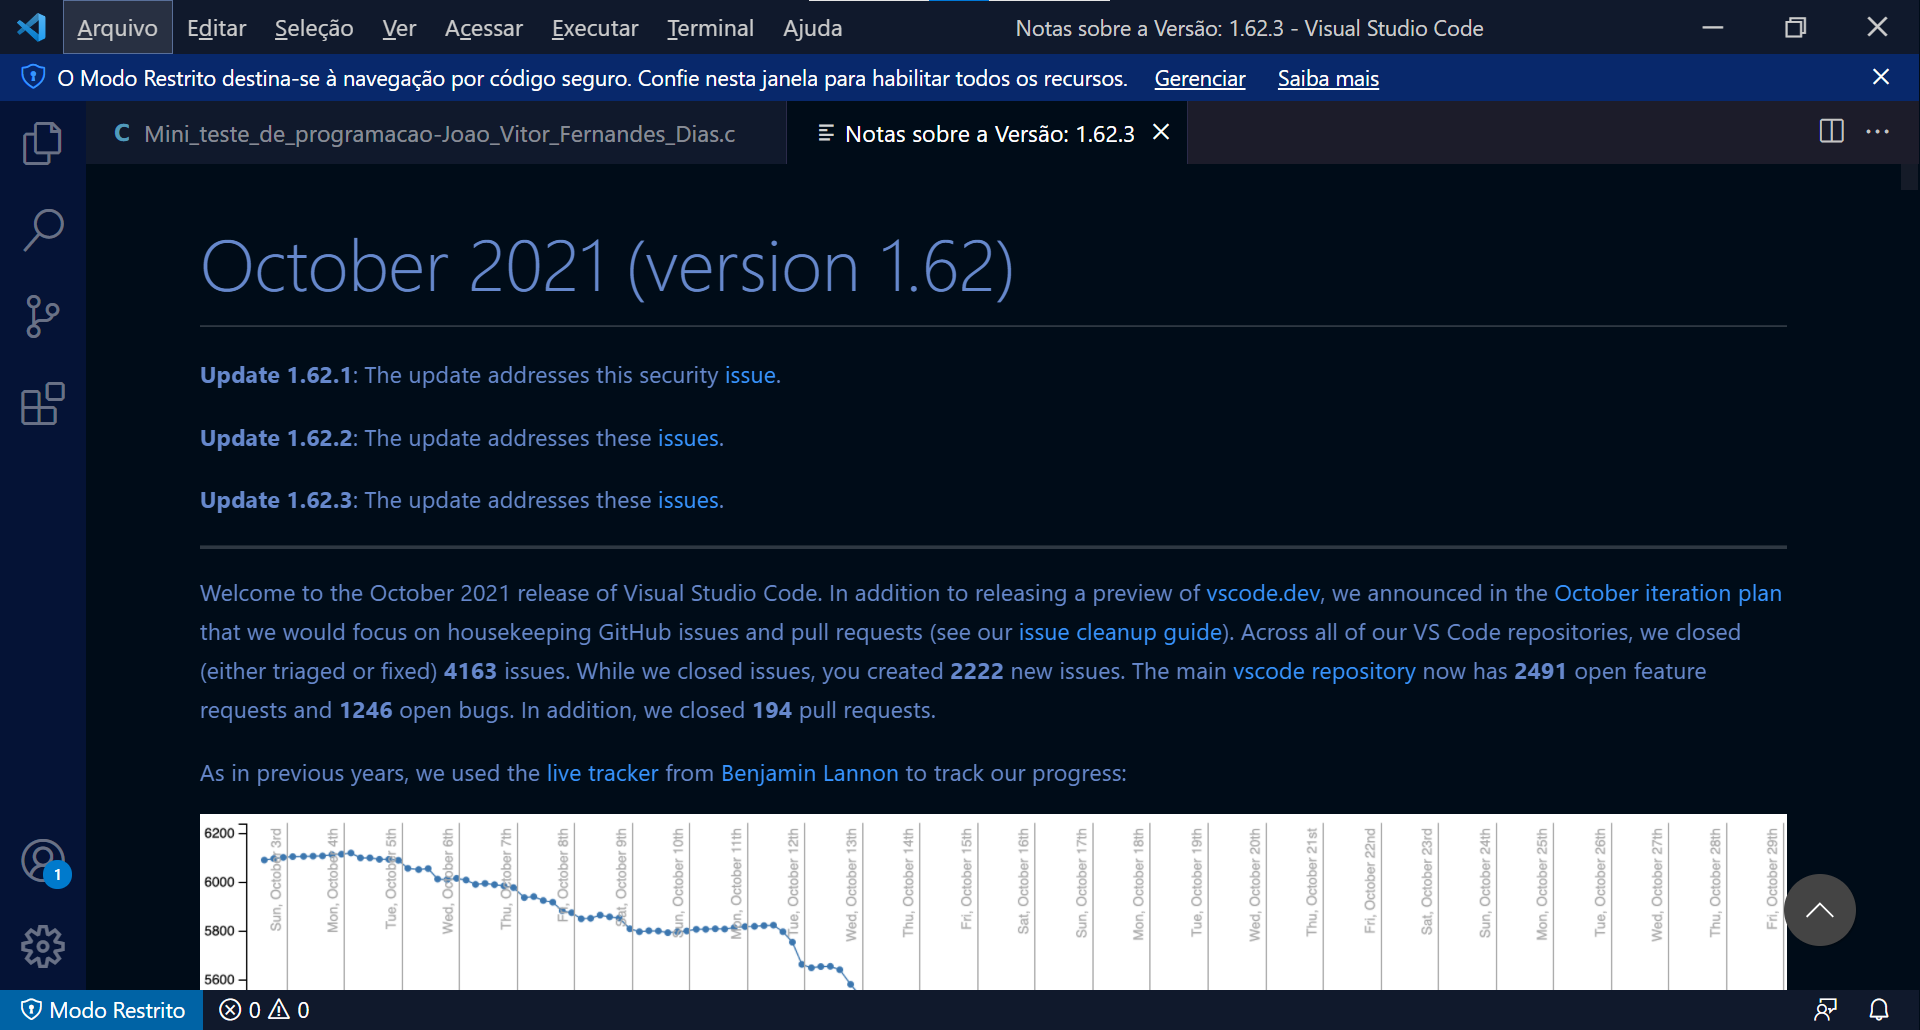
\includegraphics[width=16cm]{PicturesJoaoDias/Ferramentas/Visual Studio Code/Visual_Studio_Code-Tela_Inicial.png}
  		{\tiny \sf Fonte: autoria própria}
  	\end{figure}
  	
  \item \textit{Link de acesso:} \href{https://code.visualstudio.com/docs/?dv=win64}{Visual Studio Code} (IDE)
  	\item \textit{Versão:} 1.62.3
  	\item \textit{Descrição e comentários:}
  	  O Visual Studio Code, ou VSCode ou apenas Code, é uma IDE para programação no geral. É um dos editores de código mais utilizados atualmente, sendo ranqueado como ambiente de desenvolvimento mais popular de 2019 pelo Stack Overflow \cite{Overflow2019}. Quanto ao seu uso para a linguagem R, foi um tanto mais complicado fazê-lo funcionar do que as outras plataformas de desenvolvimento, o que é um ponto negativo. Entretanto, fazer com que o código rodasse foi surpreendentemente mais intuitivo do que nos outros. Como o VSCode pode ser utilizado para várias linguagens diferentes, é uma boa alternativa para quem busca manter todos os ambientes de desenvolvimento em um mesmo lugar. Entretanto, caso seja necessário ferramentas mais específicas do R, o RStudio ainda parece ter maior propriedade. A Figura \ref{Visual_Studio_Code} ilustra a ferramenta logo após a sua instalação.
  \end{itemize}
  		
  		\newpage
  \section{Jupyter Notebook}

  \begin{itemize}
  	
  	\item \textit{Imagem da ferramenta:}
  	
  	\begin{figure}[H]  \label{Jupyter_Notebook}
  		\centering
  		\caption{Jupyter Notebook logo após a execução}
  		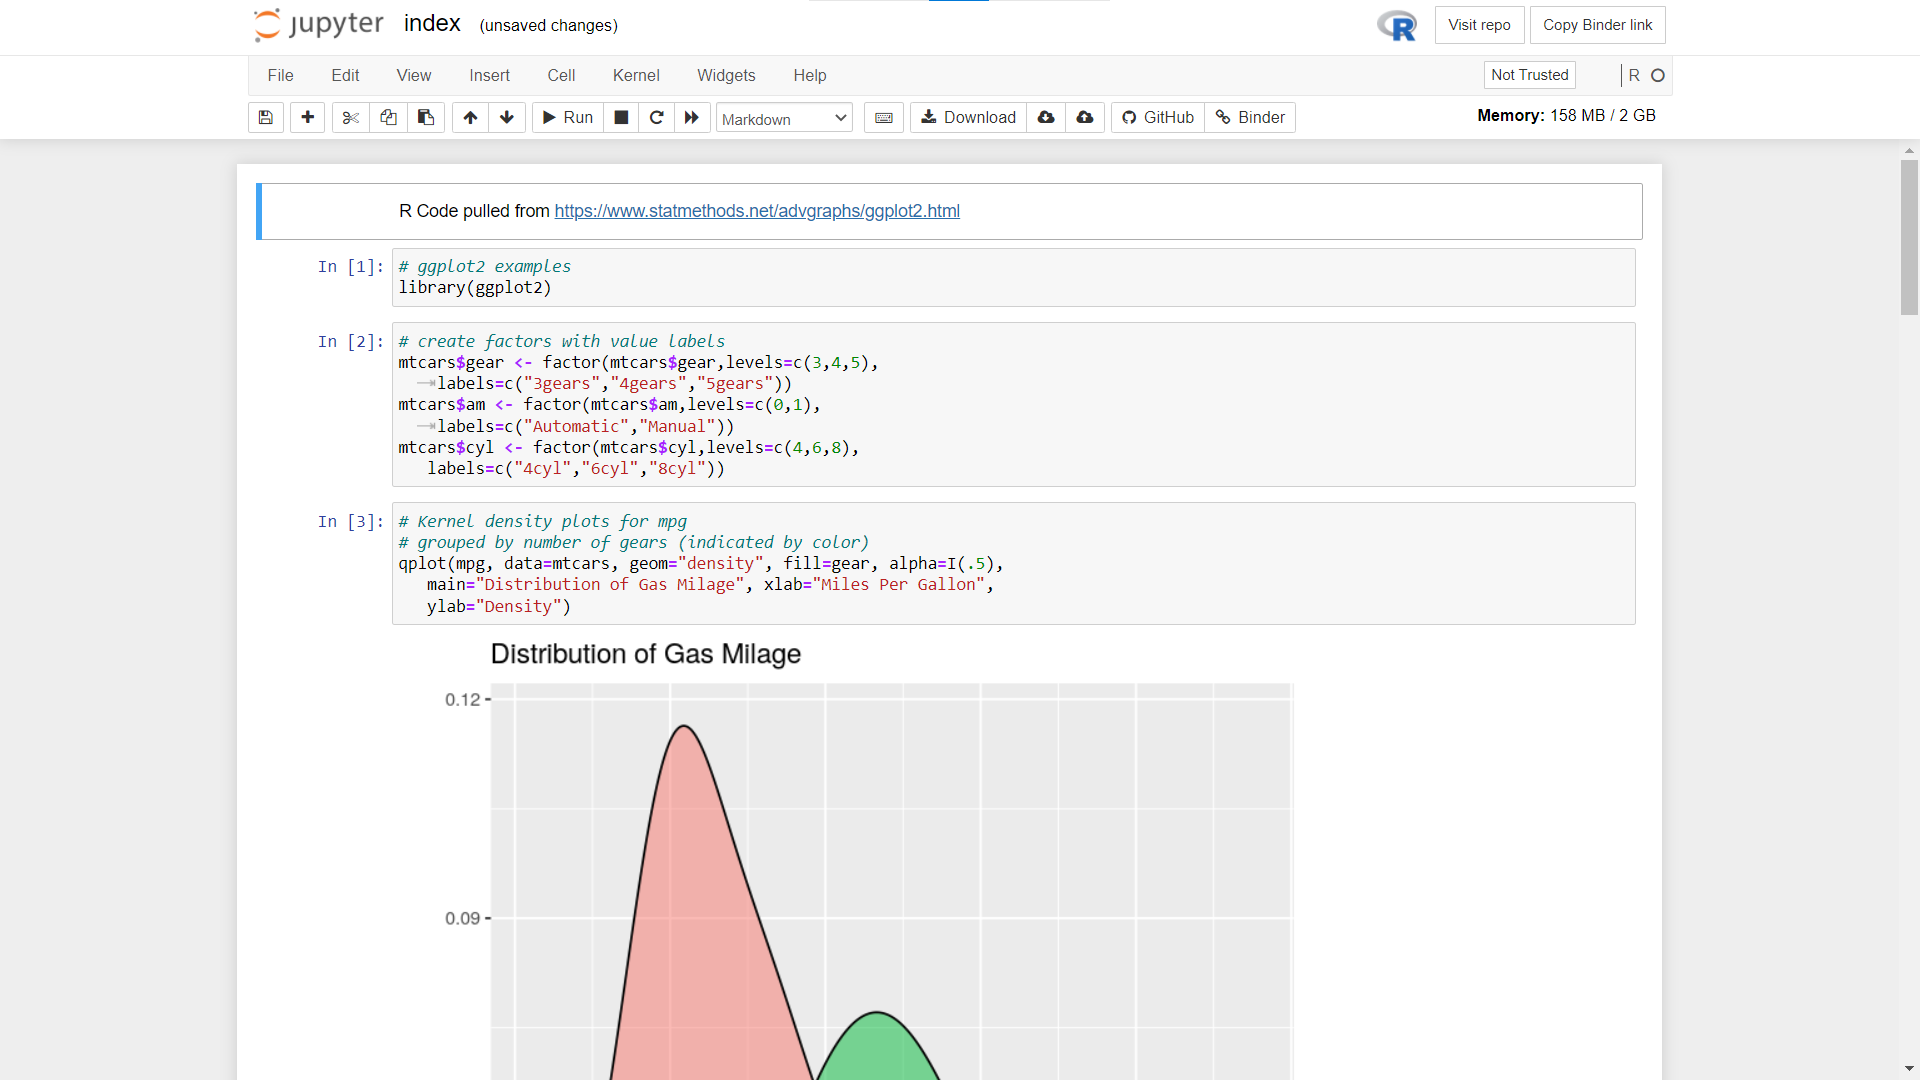
\includegraphics[width=16cm]{PicturesJoaoDias/Ferramentas/Jupyter Notebook/Jupyter_Notebook-Tela_Inicial.png}
  		{\tiny \sf Fonte: autoria própria}
  	\end{figure}
      \item \textit{Link de acesso:} \href{https://mybinder.org/v2/gh/binder-examples/r/HEAD?filepath=index.ipynb}{Jupyter notebook} (IDE e interpretador)
      \item \textit{Versões:}
      \begin{itemize}
          \item Server do notebook: 6.3.0
          \item R: 3.6.3 (2020-02-29)
      \end{itemize}
      \item \textit{Descrição e comentários:}
        Apresenta a mesma estrutura de markdown que o RStudio, porém, por aparentar ter um propósito mais geral abrangendo também códigos Python e Ruby, parece ter menos funcionalidades específicas do R o que torna ela superior na versatilidade de linguagem, mas inferior no propósito específico do uso do R. A Figura \ref{Jupyter_Notebook} ilustra a ferramenta logo após a sua execução.
        
  \end{itemize}
  \section{Resumo}
  	Além das ferramentas citadas aqui, uma maior variedade foi descrita por Milos Gregor \cite{Gregor2018} e pode ser encontrada \href{https://stagraph.com/Post?Id=31&Title=Powered+By+R}{aqui}.
  	
  	Dentre as apresentadas, para decidir de forma mais direta, escolha a IDE se você quer programar:
  	\begin{itemize}
  		\item R GUI: à moda antiga.
  		\item RStudio Desktop: apenas R de modo offline.
  		\item Rstudio Cloud: apenas R de modo online.
  		\item Visual Studio Code: várias linguagens de modo offline.
  		\item Jupyter notebook: várias linguagens de modo online.
  	\end{itemize}
  	\begin{comment}
  		Pode-se substituir a listagem acima por uma tabelinha:
  							Offline			Online
  		Apenas R			RStudio Desktop		RStudio Cloud
  		Várias linguagens	VSCode			Jupyter Notebook
  	\end{comment}



\chapterimage{Conclusao.jpg} % Chapter heading image
\chapterimage{Conclusao.jpg} % Chapter heading image
\chapter{Conclusões}
  \begin{comment}
    Prof. Dr. Ausberto S. Castro Vera
    UENF - CCT - LCMAT - Curso de Ciência da Computação
    Campos, RJ,  2021
    Disciplina: Paradigmas de Linguagens de Programação
    Os problemas enfrentados neste trabalho ...
    O trabalho que foi desenvolvido em forma resumida ...
    Aspectos não considerados que poderiam ser estudados ou úteis para ...
    
    
    \begin{figure}[H]
    	\begin{center}
    		\caption{Aplicação da Linguagem R} \label{ling2}
    		
\includegraphics[width=12cm]{R02.png} \\
    		{\tiny \sf Fonte: O autor }
    	\end{center}
    \end{figure}
  \end{comment}
  
  Como desfecho deste trabalho, vejo de forma positiva o ganho de conhecimento sobre a linguagem R e para você que leu e também a mim que escrevi. A mim foi ainda mais vantajoso pois obtive também conhecimento sobre o desenvolvimento de arquivos utilizando o \LaTeX. Percebi que durante a escrita, é complicado se ater aos "meios legado" de aquisição de conhecimento. Parte dessa dificuldade se dá por causa da facilidade e rapidez de se encontrar praticamente qualquer informação através de uma rápida pesquisa, ao invés de passar alguns minutos extras buscando PDFs online e vasculhando por todo um livro para descobrir se ele será útil para explicar uma questão específica ou não. Quanto a esta questão específica é outro ponto relevante, visto que as informações têm sido tão facilmente divulgadas nos últimos tempos, e o diálogo entre pessoas em locais distantes do globo se torno algo tão trivial, que uma boa parcela dos problemas mais comuns encontrados, principalmente na área da computação, já está bem documentada. Esses fatores acabam contribuindo para perda de parte do valor da pesquisa literária.
  
  Alguns aspectos que poderiam ter sido citados neste documento são: a visão dos programadores quanto a linguagem R em comparação a outras linguagens de propósito similar; a faixa salarial média de programadores na linguagem R por área; a explicação de como se obter os datasets apresentados no capítulo de aplicações; Uma progressão de aplicações indo do básico ao avançado.
  
  Resumidamente, temos este trabalho como um compilado básico contendo algumas informações referentes ao contexto histórico em que se encontrou a linguagem R em sua origem e seus usos na área da computação. Também são demonstradas algumas das diversas estruturas básicas e (quase) avançadas da linguagem R. Vejo que quanto aos capítulos de aplicações e ferramentas, talvez eles pudessem ter ordem inversa, sendo assim, a primeira aplicação que apresenta alguns conceitos, poderia ser mesclado aos capítulos de estruturas básicas e avançadas, assim dando uma visão um pouco mais direta de como as estruturas funcionam na prática.










\chapterimage{Bibliografia.png}
\bibliographystyle{alpha}
\bibliography{RBib}
\addcontentsline{toc}{chapter}{\textcolor{ocre}{Bibliografia}}



%----------------------------------------------------------------------------------------
\newpage
% Prof. Dr. Ausberto S. Castro Vera
% UENF - CCT - LCMAT - Curso de Ci\^{e}ncia da Computa\c{c}\~{a}o
% Campos, RJ,  2012-2019
% Disciplina: Paradigmas de Linguagens de Programa\c{c}\~{a}o
% Aluno: 


\noindent
\textbf{Disciplina:} \textit{Paradigmas de Linguagens de Programa\c{c}\~{a}o 2019}\\
\textbf{Linguagem:} \textit{Linguagem R}\\
\textbf{Aluno:} \textit{Nome Completo do aluno}\\
\textbf{Data:} \today

\section*{Ficha de avalia\c{c}\~{a}o:}



\begin{tabular}{|p{12cm}|c|}
  \hline
  % after \\: \hline or \cline{col1-col2} \cline{col3-col4} ...
  \textbf{Aspectos de avalia\c{c}\~{a}o (requisitos m\'{\i}nimos)} & \textbf{Pontos} \\
  \hline
  Elementos b\'{a}sicos da linguagem (M\'{a}ximo: 01 pontos) &  \\
  $\bullet$ Sintaxe (vari\'{a}veis, constantes, comandos, opera\c{c}\~{o}es, etc.) &  \\
  $\bullet$ Usos e \'{a}reas de Aplica\c{c}\~{a}o da Linguagem &  \\
  \hline
  Cada elemento da linguagem (defini\c{c}\~{a}o) com exemplos (M\'{a}ximo: 02 pontos) &  \\
  $\bullet$ Exemplos com fonte diferenciada ( Courier , 10 pts, azul) & \\
  \hline
  M\'{\i}nimo 5 exemplos completos - Aplica\c{c}\~{o}es (M\'{a}ximo : 2 pontos) &  \\
  $\bullet$ Uso de rotinas-fun\c{c}\~{o}es-procedimentos, E/S formatadas &  \\
  $\bullet$ Menu de opera\c{c}\~{o}es, programas gr\'{a}ficos, matrizes, aplica\c{c}\~{o}es &  \\
  \hline
  Ferramentas (compiladores, interpretadores, etc.) (M\'{a}ximo : 2 pontos) &  \\
  $\bullet$ Ferramentas utilizadas nos exemplos: pelo menos DUAS&  \\
  $\bullet$ Descri\c{c}\~{a}o de Ferramentas existentes:  m\'{a}ximo 5&  \\
  $\bullet$ Mostrar as telas dos exemplos junto ao compilador-interpretador&  \\
  $\bullet$  Mostrar as telas dos resultados obtidos nas ferramentas &  \\
  $\bullet$ Descri\c{c}\~{a}o das ferramentas (autor, vers\~{a}o, homepage, tipo, etc.) &  \\
  \hline
  Organiza\c{c}\~{a}o do trabalho (M\'{a}ximo: 01 ponto) &  \\
  $\bullet$ Conte\'{u}do, Historia, Se\c{c}\~{o}es, gr\'{a}ficos, exemplos, conclus\~{o}es, bibliografia &  \\
  \hline
   Uso de Bibliografia (M\'{a}ximo: 01 ponto)&  \\
   $\bullet$ Livros: pelo menos 3&  \\
   $\bullet$ Artigos cient\'{\i}ficos: pelo menos 3 (IEEE Xplore, ACM Library)&  \\
   $\bullet$ Todas as Refer\^{e}ncias dentro do texto, tipo [ABC 04] & \\
   $\bullet$ Evite Refer\^{e}ncias da Internet & \\
   \hline
     &  \\
  Conceito do Professor (Opcional: 01 ponto) & \\
  \hline
   & \\
  \hfill Nota Final do trabalho: & \\
  \hline
\end{tabular}\\
\textit{Observa\c{c}\~{a}o:} Requisitos m\'{\i}nimos significa a \textit{metade} dos pontos


\end{document}

